\documentclass[
  amsfonts,
  amsmath,
  tbtags,
  amssymb,
  aps,
  nobibnotes,
  %% prl,
  twocolumn,
  superscriptaddress,
]{revtex4-2}

% imports
\usepackage{appendix}[titletoc]
\usepackage[english]{babel}
\usepackage[justification=centering]{caption}
\usepackage{float}
\usepackage{graphicx}
\usepackage{hyperref}
\usepackage[utf8]{inputenc}
\usepackage{layouts}
\usepackage{optidef}
\usepackage{physics}
\usepackage{setspace}
\usepackage[labelformat=simple]{subcaption}
\usepackage{xcolor}

% configure imports
\DeclareMathOperator*{\argmin}{arg\,min}
\newcommand{\todo}[1]{\textcolor{red}{TODO: #1}}
\definecolor{darkgreen}{RGB}{46, 184, 46}
\newcommand{\half}{\frac{1}{2}}
\newcommand{\R}{\mathbb{R}}
\captionsetup[subfigure]{labelformat=empty, skip=0pt}
\restylefloat{table}
\renewcommand\thesubfigure{(\alph{subfigure})}



\begin{document}


%% TITLE
\title{Robust Control of a Fluxonium Qubit}

\author{Thomas Propson}
\email{tcpropson@uchicago.edu}
\affiliation{
  James Franck Institute, University of Chicago, Chicago, Illinois 60637, USA
}
\affiliation{
  Department of Physics, University of Chicago, Chicago, Illinois 60637, USA
}
\author{Brian Jackson}
\author{Zac Manchester}
\affiliation{
  Department of Aeronautics and Astronautics Engineering, Stanford University, 496 Lomita Mall, Stanford, CA 94305
}
\author{David I. Schuster}
\affiliation{
  James Franck Institute, University of Chicago, Chicago, Illinois 60637, USA
}
\affiliation{
  Department of Physics, University of Chicago, Chicago, Illinois 60637, USA
}
\affiliation{
  Pritzker School of Molecular Engineering, University of Chicago, Chicago, Illinois 60637, USA
}

\date{\today}

%% TITLE
\title{Robust Trajectory Optimization on a Quantum System}

\author{Thomas Propson}
\email{tcpropson@uchicago.edu}
\affiliation{
  James Franck Institute, University of Chicago, Chicago, Illinois 60637, USA
}
\affiliation{
  Department of Physics, University of Chicago, Chicago, Illinois 60637, USA
}
\author{Brian Jackson}
\author{Zachary Manchester}
\affiliation{
  Robotics Institute, Carnegie Mellon University, Pittsburgh, Pennsylvania 15213, USA
}
\author{David I. Schuster}
\affiliation{
  James Franck Institute, University of Chicago, Chicago, Illinois 60637, USA
}
\affiliation{
  Department of Physics, University of Chicago, Chicago, Illinois 60637, USA
}
\affiliation{
  Pritzker School of Molecular Engineering, University of Chicago, Chicago, Illinois 60637, USA
}

\date{\today}

%% ABSTRACT
\begin{abstract}
  The ability to engineer high-fidelity gates on quantum processors in the presence of
  systematic errors remains the primary challenge requisite to achieving quantum advantage.
  Quantum optimal control methods have proven effective in experimentally
  realizing high-fidelity gates, but they require exquisite calibration to be performant.
  We apply robust trajectory optimization techniques to suppress gate errors arising from system
  parameter uncertainty.
  We propose a method that takes advantage of uncertain parameter
  derivative information while maintaining
  computational efficiency by transforming high-order differential equations to coupled,
  first-order ODEs.
  Additionally, the effect of depolarization on a gate is most accurately modeled by
  integrating the Lindblad master equation,
  which is computationally expensive.
  We propose a computationally efficient model
  and utilize time-optimal control to achieve high fidelity gates in the presence of depolarization.
  We apply these techniques to a two level approximation of a fluxonium qubit and suppress
  simulated gate errors due to parameter uncertainty below $10^{-7}$ for
  static parameter deviations on the order of $1\%$.
\end{abstract}

\maketitle


\maketitle

\section{Introduction}
Quantum optimal control (QOC) techniques are a class of optimization
algorithms for accurately and efficiently manipulating quantum systems.
Early techniques were proposed for nuclear magnetic resonance experiments
\cite{vandersypen2005nmr, kehlet2004improving, khaneja2005optimal,
  maximov2008optimal, nielsen2010optimal, skinner2003application, tosner2009optimal},
and applications now include superconducting circuits \cite{abdelhafez2020universal,
  chakram2020multimode, fisher2010optimal, gokhale2019partial,
  huang2020engineering, leng2019robust, leung2017speedup, li2020fast,
  xu2020nonadiabatic},
neutral atoms and ions \cite{brouzos2015quantum,
  de2008optimal, goerz2011quantum, guo2019high, jensen2019time,
  larrouy2020fast, omran2019generation, rosi2013fast, sorensen2019qengine,
  treutlein2006microwave, van2016optimal},
nitrogen-vacancy centers in diamond \cite{chou2015optimal,
  dolde2014high, geng2016experimental,
  nobauer2015smooth, poggiali2018optimal, rembold2020introduction, tian2019optimal},
and Bose-Einstien condensates \cite{amri2019optimal, sorensen2018quantum}.
For quantum computation,
optimal control techniques are employed to achieve high fidelity gates
while adhering to experimental constraints.
Experimental errors may cause the system to deviate
from the model used in optimization, leading
to poor experimental performance.
Robust control techniques improve upon
standard optimal control techniques by encoding
model uncertainties
in optimization objectives, yielding performance
guarantees over a range of parameters \cite{Zhou97,Morimoto00,Manchester18}.
We adapt robust control techniques from the robotics community to mitigate
realistic model uncertainties for
a superconducting fluxonium qubit.

QOC techniques have had tremendous success in
engineering high fidelity quantum gates \cite{
  chou2015optimal, dolde2014high, egger2013optimized, egger2014adaptive,
  grace2007optimal, heeres2017implementing, huang2014optimal,
  kelly2014optimal, leng2019robust, liebermann2016optimal,
  nebendahl2009optimal, rebentrost2009optimal, rebentrost2009optimal2,
  spiteri2018quantum, sporl2007optimal}. 
While standard QOC techniques can predict system behavior
with high accuracy, they are sensitive to experimental
errors such as parameter drift, noise, finite control 
resolution, and decoherence. Multiple techniques have been developed to address
these shortcomings. Analytic techniques to mitigate parameter deviation errors
include dynamic and geometric phase considerations
\cite{han2020experimental, xu2020nonadiabatic} and
composite pulses \cite{cummins2000use, cummins2003tackling,
  kupce1995stretched, merrill2014progress}.
To mitigate decoherence, Floquet techniques have been employed
\cite{huang2020engineering, mundada2020floquet}.
Numerical techniques to mitigate parameter deviation errors
include closed-loop methods \cite{egger2014adaptive, feng2018gradient, huang2020engineering,
  wittler2020integrated} and open-loop methods \cite{
  allen2019robust, carvalho2020error, reinhold2019controlling,
  rembold2020introduction, kosut2013robust}.
Numerical techniques to mitigate decoherence include
modeling master equations \cite{rembold2020introduction} and employing
Monte Carlo style quantum trajectories \cite{abdelhafez2019gradient}.

In this work, we study three robust control techniques that
make the system's state trajectory less sensitive
to static and time-dependent parameter deviations:
\begin{enumerate}
  \item A sampling method, similar to the work of \cite{allen2019robust,
    carvalho2020error, reinhold2019controlling, rembold2020introduction}.
  \item An unscented sampling method adapted from the unscented transform used in the 
    state estimation community \cite{howell2020direct, julier2004unscented,
      lee2013sigma, manchester2016derivative}.
  \item A derivative-penalization method, which uses efficient mixed-mode differentiation
    to compute derivative information of parameter deviations with respect to the 
    quantum state trajectory.
\end{enumerate}
We apply these techniques to the fluxonium qubit presented in \cite{zhang2020universal}.
We also show that QOC can solve important problems for fluxonium-based qubits,
in particular, taking advantage of the $T_{1}$-dependence of the controls
to mitigate longitudinal relaxation type decoherence and
performing phase gates in arbitrary times.
To mitigate errors due to longitudinal
relaxation, we perform time-optimal control and
utilize an efficient optimization objective that does
not pay the increased computational cost of integrating a master equation.
Leveraging recent advances in trajectory optimization within the field of robotics, we
solve these optimization problems using the ALTRO solver, which uses iterative LQR 
(iLQR)---a differential-dynamic programming (DDP)-based indirect method similar to shooting
methods such as GOAT \cite{machnes2015gradient}, GRAPE
\cite{khaneja2005optimal, leung2017speedup}, and Krotov's \cite{goerz2019krotov}---within 
an augmented Lagrangian framework to handle nonlinear equality and inequality constraints at 
each time step \cite{howell2019altro}. 

This paper is organized as follows.
First, we introduce the ALTRO method in the context of QOC
in Section \ref{sec:background}.
We describe realistic constraints for the fluxonium and
map them to the ALTRO method in Section \ref{sec:fluxonium}. Then, we
outline a method for making the optimization aware of longitudinal
relaxation in Section \ref{sec:longitude}. Next, we outline three methods for achieving
robustness to static parameter deviations in Section \ref{sec:static}. Finally,
we employ the robust control techniques to mitigate 1/$f$ flux noise
in Section \ref{sec:stochastic}.

\section{Background \label{sec:background}}
In this section, we
review the QOC problem statement
and describe the ALTRO solver \cite{howell2019altro}.
QOC concerns a vector of time-dependent control parameters $u(t)$
that steer the evolution of a (quantum) state $\ket{\psi(t)}$.
The evolution of the state is governed by the time-dependent
Schr{\"o}dinger equation (TDSE),
\begin{equation}
  i \hbar \frac{d}{dt} \ket{\psi(t)} = H(u(t), t) \ket{\psi(t)}.
  \label{eq:tdse}
\end{equation}
The Hamiltonian $H(u(t), t)$ is determined by the quantum system.
The QOC problem is to find the
controls that minimize a functional $J(u(t))$.
To make the problem numerically tractable,
the controls and state are discretized into $N$ time steps.
In the case of a single state-transfer problem, the functional is
the infidelity of the target state and the initial state evolved
to the final time step,
$J(u) = 1 - {\lvert \braket{\psi_{f}}{\psi_{N}(u)} \rvert}^{2}$.
In general, $J(u)$ is a linear combination of cost functions on the state
as well as cost functions on the controls.
Standard QOC solvers compute derivatives of the functional $\nabla_{u} J(u)$,
which can easily be used to implement first-order optimization methods
\cite{machnes2015tunable, khaneja2005optimal, leung2017speedup, goerz2019krotov}.

Alternatively, the QOC problem can be formulated as a trajectory optimization problem 
and solved using a variety of specialized solvers developed by the robotics community
\cite{Schulman13, Tedrake16, Hereid2017FROST, howell2019altro}.
The functional $J(u)$ is divided into its constituent
cost functions at each time step $\ell_{k}(x_{k}, u_{k})$,
where $k \in \{1, ..., N\}$ denotes the time step,
$x_{k}$ is the augmented state vector,
and $u_{k}$ is the augmented control vector.
The augmented state contains all relevant variables
that are dependent upon the controls, for example the state
$\ket{\psi_{k}} \subseteq x_{k}$.
The augmented state trajectory obeys the physics of the system if
the dynamics constraint is satisfied
$x_{k + 1} = f(x_{k}, u_{k})$. For QOC, the discrete
dynamics function $f(x_{k}, u_{k})$ propagates the state by
integrating the TDSE \eqref{eq:tdse} with Runge-Kutta methods \cite{jorgensen2011numerical}
or exponential integrators \cite{auer2018magnus, berland2006solving, einkemmer2017performance,
shillito2020fast}.

Additional constraints on the augmented controls and augmented states
are encoded in constraint functions.
The constraint functions are put into a form such that, when the constraint is satisfied,
inequality constraint functions obey $g_{k}(x_{k}, u_{k}) \leq 0$ and
equality constraint functions obey $h_{k}(x_{k}, u_{k}) = 0$. The constraint
functions may be vector-valued to encode multiple constraints of each type.
The constraint function's violation is the magnitude by which it is not satisfied:
$\textrm{max}(g(\cdot), 0)$ or $\textrm{max}(\abs{h(\cdot)})$
where $\textrm{max}(\cdot)$ and $\abs{\cdot}$ act element-wise.
Stated concisely, the trajectory optimization problem is,
\begin{mini!}[2]
  {x_{1:N},u_{1:N-1}}{\ell_{N}(x_N) + \sum_{k=1}^{N-1}
    \ell_{k}(x_k,u_k)}{}{} \label{eq:gcostfun}
    \addConstraint{x_{k+1} = f(x_k,u_k) \ \forall \ k} \label{eq:gdyncon}
    \addConstraint{g_k(x_k,u_k) \leq 0 \ \forall \ k} \label{eq:ineqcon}
    \addConstraint{h_k(x_k,u_k) = 0 \ \forall \ k.} \label{eq:eqcon}
\end{mini!}

Standard techniques for solving \eqref{eq:gcostfun}-\eqref{eq:eqcon} typically
fall into two categories: direct methods \cite{Hargraves87, kelly2017introduction}
and indirect methods \cite{betts1998survey}. For indirect methods,
the augmented controls are the decision variables--the
variables the optimizer adjusts to solve the problem.
The augmented states are obtained from the augmented controls using the discrete dynamics function,
and are then used to evaluate derivatives of the cost functions \eqref{eq:gcostfun}.
Then, the derivative information is employed to update the augmented controls.
This approach is taken by standard QOC solvers such as GOAT \cite{machnes2015tunable},
GRAPE \cite{khaneja2005optimal, leung2017speedup}, and Krotov's method \cite{goerz2019krotov}.
Conversely, direct methods treat both the augmented controls and the augmented states as decision
variables. In addition to minimizing the cost functions, the optimizer uses derivative information
for the discrete dynamics function
to satisfy the dynamics constraint \eqref{eq:gdyncon} to a specified tolerance.
In this sense, the TDSE \eqref{eq:tdse} is a constraint that may be violated
for intermediate steps of the optimization, where the states need not be physical.
The direct approach lends itself to a nonlinear program formulation, for which
a variety of general-purpose solvers exist \cite{gill2005snopt, wachter2006implementation}.
Recent state-of-the-art solvers, such as ALTRO,
have combined principles from both of these approaches. ALTRO uses an
iterative linear-quadratic regulator (iLQR) algorithm
\cite{Li2004a} as the internal solver of an augmented Lagrangian method (ALM)
\cite{lantoine2012hybrid, plancher2017constrained, nocedal2006numerical}
and employs a projected Newton method \cite{bertsekas1982projected, rao1998application}
in its final solving stage.

iLQR is an indirect method
for solving the dynamically constrained
trajectory optimization problem \eqref{eq:gcostfun}-\eqref{eq:gdyncon},
and its update procedure is based on the differential-dynamic-programming approach
\cite{mayne1966a}.
First, iLQR uses an initial guess for the augmented controls to obtain the augmented
states with the discrete dynamics function.
iLQR then constructs quadratic models for each cost function using
their zeroth-, first- and second-order derivatives in a Taylor expansion
about the current augmented controls and augmented states.
These models are used to derive a recurrence relation between time steps
that gives the locally optimal update for the augmented controls.
Finally, a line search \cite{zhang2006global}
is performed in the direction of this update to ensure a
decrease in the objective \eqref{eq:gcostfun}. This procedure
is repeated until convergence.

Indirect solvers such as iLQR are popular
because they are very computationally efficient and maintain
high accuracy for the discrete dynamics throughout the optimization.
However, standard implementations cannot handle
nonlinear equality and inequality
constraints \eqref{eq:ineqcon}-\eqref{eq:eqcon}.
Projected gradient methods are a typical approach
to handle constraints
\cite{clarkson2010coresets, hauswirth2016projected, morzhin2019minimal,
  nikolskii2007convergence}. Unfortunately, within the indirect framework,
they can only be used for constraints on the augmented controls,
not the augmented states.
Another technique, which is popular for QOC \cite{heeres2017implementing, leung2017speedup,
reinhold2019controlling},
is to add the constraint functions to the objective.
This strategy does not guarantee that the constraints
are satisfied as the solver trades
minimization of the cost functions and constraint functions against each other.
ALM remedies this issue by adaptively adjusting a Lagrange multiplier estimate
for each constraint function to ensure the constraints are satisfied.
ALM adds terms that are linear and quadratic in the constraint functions
to the objective. Then, the new objective is minimized with
iLQR. If the solution obtained with iLQR does not satisfy the constraints,
the prefactors for the constraint terms in the objective are increased
intelligently and the procedure is repeated.

ALM converges superlinearly, but poor numerical conditioning may lead
to small decreases in the constraint violations near the locally optimal solution
\cite{bertsekas1996constrained}.
To address this shortcoming, ALTRO
projects the solution from the ALM stage onto the constraint manifold using
a (direct) projected Newton method, achieving ultra-low
constraint violations $\sim 10^{-8}$.
For more information on the details of the ALTRO
solver, see \cite{howell2019altro, Jackson2020altroc}.

As opposed to standard QOC solvers, ALTRO
can satisfy constraints
on both the augmented controls and the augmented states to tight tolerances.
This advantage is crucial for this work, where multiple medium-priority cost functions
are minimized subject to many high-priority constraints.

\section{QOC for the Fluxonium \label{sec:fluxonium}}
In the following, we optimize quantum gates
for the superconducting fluxonium qubit -- a promising
building block for quantum computers due to its high
coherence times
\cite{earnest2018realization, lin2018demonstration,
  manucharyan2009fluxonium, somoroff2021millisecond, nguyen2019high,
  zhang2020universal}.
In this section, we use the trajectory optimization
formalism \eqref{eq:gcostfun}-\eqref{eq:eqcon}
to define the optimization problem \eqref{eq:costfun}-\eqref{eq:ic_con},
which we extend in subsequent sections to account
for experimental error channels.
To high accuracy, we approximate the fluxonium Hamiltonian near the flux-frustration
point as a two-level system:
\begin{align}
  H/h &= f_{q} \frac{\sigma_{z}}{2} + a(t) \frac{\sigma_{x}}{2}.
  \label{eq:hamiltonian}
\end{align}
Here, $f_{q}$ is the qubit frequency at the flux-frustration point,
$a(t)$ is the control governing the flux offset from the flux-frustration point,
$h$ is Planck's constant, and $\sigma_{z}, \sigma_{x}$
are Pauli matrices. Although the coherent dynamics can be described with this two-level
system model, our noise model, experimental constraints, and system parameters
consider the full system, and they are representative of the fluxonium
presented in \cite{zhang2020universal}.

First, we introduce the augmented control and state for the fluxonium gate problem.
Since the ALTRO implementation we use does not currently
support complex numbers, we represent the quantum states
in the isomorphism $\mathcal{H}(\mathbb{C}^{n})
\cong \mathcal{H}(\mathbb{R}^{2n})$ given in \cite{leung2017speedup},
\begin{equation}
  H \ket{\psi} \cong \begin{pmatrix} H_{\textrm{re}} & -H_{\textrm{im}}
    \\ H_{\textrm{im}} & H_{\textrm{re}}\end{pmatrix}
  \begin{pmatrix} \ket{\psi}_{\textrm{re}} \\ \ket{\psi}_{\textrm{im}}\end{pmatrix}.
  \label{eq:isomorphism}
\end{equation}
We use $\psi$ -- abandoning bra-ket notation -- to denote the real representation of a state
given by the right-hand-side of \eqref{eq:isomorphism}.
To refer to the discrete moments of the flux, we introduce the notation
$\int_{t} a_{k} \equiv \int^{t_{k}}_{t_{1}} a(t) \ \mathrm{d}t$,
$a_{k} \equiv a(t_{k})$,
$\mathrm{d}^{n}_{t} a_{k} \equiv \mathrm{d}^{n}a(t)/{\mathrm{d}t}^{n} \lvert_{t = t_{k}}$.
The augmented control and state are:
\begin{equation}
  \begingroup
  \renewcommand*{\arraystretch}{1.3}
  \mathbf{u}_{k} = \begin{pmatrix} \mathrm{d}^{2}_{t} a_{k} \end{pmatrix}, \quad
  \mathbf{x}_{k} = \begin{pmatrix} \psi^{0}_{k} \\ \psi^{1}_{k}
    \\ \int_{t} a_{k} \\ a_{k} \\ \mathrm{d}_{t} a_{k} \end{pmatrix}.
  \endgroup
  \label{eq:astatecontrols}
\end{equation}
Here, the superscript on the quantum states $i \in \{0, 1\}$ acts as a label.
In standard QOC frameworks, the derivatives of the control fields
are obtained with finite difference methods, e.g.,
$\mathrm{d}_{t} a_{k} \approx (a_{k + 1} - a_{k}) / \Delta t$ \cite{leung2017speedup}.
Because ALTRO requires that cost functions do not use information from multiple time steps,
we make $\mathrm{d}^{2}_{t} a_{k}$ a decision variable and
numerically integrate coupled ODEs to obtain $\mathrm{d}_{t} a_{k}$, $a_{k}$, and $\int_{t} a_{k}$
so that we may penalize them in cost functions.
Similarly, the quantum states are obtained by numerically integrating
the TDSE \eqref{eq:tdse} with the fluxonium Hamiltonian \eqref{eq:hamiltonian}
and the given flux $a_{k}$. These numerical integration rules are implemented
in the discrete dynamics function for the problem, and they give rise to the
dynamics constraint \eqref{eq:dyn_con}.

Next, we outline the constraints for this problem.
Casting this problem in terms of a multi-state transfer problem, we fix as the initial states
 $\ket*{\psi^{0}_{1}} = \ket*{0}$, $\ket*{\psi^{1}_{1}} = \ket*{1}$
\eqref{eq:istate_con}.
The states at the final time step are constrained to be
the target states $\ket*{\psi^{i}_{N}} = \ket*{\psi^{i}_{T}} \equiv
U \ket*{\psi^{i}_{1}} \ \forall \ i$
\eqref{eq:tstate_con} where $U = X/2, Y/2, Z/2$ denotes the target gate.
Furthermore, we impose the normalization constraint
${\lvert \braket*{\psi^{i}_{k}}{\psi^{i}_{k}} \rvert}^{2} = 1 \ \forall \ i,k$
\eqref{eq:statenorm_con}
to ensure the solver does not take advantage of discretization errors in numerical integration.
For the flux moments,
we have the initial condition $\int_{t} a_{1} = \mathrm{d}_{t} a_{1} = 0$
\eqref{eq:ic_con}.
We also enforce the boundary condition $a_{1} = a_{N} = 0$ \eqref{eq:ic_con}, \eqref{eq:znf_con}
so the gates may be concatenated arbitrarily. 
We impose the zero net-flux constraint $\int_{t} a_{N} = 0$
\eqref{eq:znf_con}
which mitigates the inductive drift ubiquitous in flux-bias lines
\cite{battistel2019fast, krantz2019quantum, zhang2020universal}.
Additionally, the flux is constrained by $\lvert a_{k} \rvert \leq 0.5 \ \textrm{GHz}
\ \forall \ k$ \eqref{eq:amp_con} to ensure the two-level approximation
\eqref{eq:hamiltonian} remains valid. Above $0.5$ GHz,
we experimentally observe that the relationship
between the energy levels and the flux becomes strongly non-linear.
All gates presented in this work satisfy these constraints to
a maximum violation of $\sim 10^{-8}$.

The cost function at each time step is
$\ell_{k}(\mathbf{x}_{k}, \mathbf{u}_{k}) = (\mathbf{x}_{k}
- \mathbf{x}_{T})^{T} Q_{k} (\mathbf{x}_{k} - \mathbf{x}_{T})
+ \mathbf{u}^{T}_{k} R_{k} \mathbf{u}_{k}$
where $Q_{k}$ and $R_{k}$ are diagonal matrices
of hyperparameters that assign weights to cost function contributions.
The $Q_{k}$ term
penalizes deviations from the target augmented state
$\mathbf{x}_{T} = (\psi^{0}_{T}, \psi^{1}_{T}, 0, 0, 0)^{T}$,
which is consistent with the constraints we have
imposed on $\ket*{\psi^{i}_{N}}$, $\int_{t} a_{N}$, and $a_{N}$.
Accordingly, this term penalizes the squared
difference of $\psi^{i}_{k}$ and $\psi^{i}_{T}$
and penalizes the norm of $\int_{t} a_{k}$, $a_{k}$, and $\mathrm{d}_{t} a_{k}$.
We penalize the squared difference of the final and target
quantum states, rather than their infidelities,
because the Hessian of the squared-difference cost function is diagonal -- which
makes matrix multiplications fast -- and we wish to optimize $Z/2$ gates,
which requires a metric that is sensitive to global phases for the initial
states $\ket*{0}$ and $\ket*{1}$.
Additionally, the $R_{k}$ term penalizes the norm of $\mathrm{d}^{2}_{t} a_{k}$.
Penalizing the norm of $\mathrm{d}^{2}_{t} a_{k}$ and $\mathrm{d}_{t} a_{k}$
makes $a_{k}$ smooth, which mitigates high-frequency AWG transitions.
Stated succinctly, the optimization problem takes the form:
\begin{mini!}[2] 
  {\substack{\mathbf{x}_1,\ldots,\mathbf{x}_N \\ \mathbf{u}_1,\ldots,\mathbf{u}_{N-1}}}
  {\sum_{k=1}^N {(\mathbf{x}_k-\mathbf{x}_{T})}^{T} Q_k (\mathbf{x}_k-\mathbf{x}_{T})
    + \sum_{k=1}^{N-1} {\mathbf{u}_k}^{T} R_k \mathbf{u}_{k}}{}{} \label{eq:costfun}
  \addConstraint{\mathbf{x}_{k+1}}{= \mathbf{f}(\mathbf{x}_k, \mathbf{u}_k) \ \forall \ k}
  \label{eq:dyn_con}
  \addConstraint{\ket*{\psi^{0}_{1}} = \ket*{0}, \ket*{\psi^{1}_{1}} = \ket*{1}}
  \label{eq:istate_con}
  \addConstraint{{\textstyle \int_{t}} a_{1} = a_{1} = \mathrm{d}_{t} a_{1} = 0}
  \label{eq:ic_con}
  \addConstraint{\ket*{\psi^{i}_{N}} = \ket*{\psi^{i}_{T}}
    \ \forall \  i} \label{eq:tstate_con}
  \addConstraint{{\textstyle \int_{t}} a_{N} = a_{N} = 0} \label{eq:znf_con}
  \addConstraint{{\lvert \braket{\psi^{i}_{k}}{\psi^{i}_{k}}
      \rvert}^{2} = 1 \ \forall \ i, k} \label{eq:statenorm_con}
  \addConstraint{|a_{k}| \leq 0.5 \ \textrm{GHz} \ \forall \ k.} \label{eq:amp_con}
\end{mini!}

Next, we remark on our problem formulation.
We put a cost function at all time steps
because it benefits the iLQR solving stage \cite{Jackson2020altroc};
although this may incentivize early achievement of the desired gate,
as in Ref. \cite{leung2017speedup}, we are primarily concerned
with achieving the gate at the final time step, which the target-state
constraint \eqref{eq:tstate_con} ensures.
Additionally, the target-state constraint
requires the final state to match the target state, including its global phase,
up to our chosen maximum constraint violation $\sim 10^{-8}$.
If we did not impose this constraint, the optimizer would be
allowed to sacrifice the closed-system gate error to achieve better
performance on the other cost functions, which is undesirable.
To enforce a constraint in standard QOC frameworks,
the prefactor for the constraint function is manually increased
between separate optimization instances until the constraint is satisfied
\cite{heeres2017implementing, leung2017speedup, reinhold2019controlling},
which becomes infeasible for more than one constraint.
ALM automates these prefactor updates to find
a solution that satisfies all of the given constraints.
Hence, ALTRO's ability to handle multiple constraints makes it
an attractive solver for QOC problems.

In extraordinarily difficult cases of
QOC, it may be impossible
to obey the physics of the system and achieve the desired gate \cite{abdelhafez2020universal},
i.e., the dynamics constraint \eqref{eq:dyn_con}
and the target-state constraint \eqref{eq:tstate_con} may be mutually unsatisfiable.
In this case, the prefactors for the constraint function terms
in the ALM objective will tend to infinity -- leading to numerical instability -- and the
optimization will not converge. To maintain a constrained approach in this situation,
the maximum constraint violation for the target-state constraint can be raised
to a level commensurate with the minimum acceptable gate error.

Finally, for ALTRO's first indirect stage,
the augmented states are obtained explicitly with the discrete
dynamics function, so the dynamics constraint and initial conditions
\eqref{eq:dyn_con}-\eqref{eq:ic_con} are satisfied by construction.
In this stage, the rest of the constraint functions \eqref{eq:tstate_con}-\eqref{eq:amp_con}
are added to the objective in their isomorphism-equivalent form \eqref{eq:isomorphism}.
Conversely, for the second direct stage, all of the constraints
\eqref{eq:dyn_con}-\eqref{eq:amp_con} are used to define
the projection onto the constraint manifold, and the objective is unmodified.
Hence, the quantum states become
free parameters that are adjusted to satisfy the TDSE.
Although the final solution's deviation from the TDSE is never
more than the maximum constraint violation,
we explicitly integrate the TDSE when reporting gate errors to ensure accuracy.
Exploring the benefit of direct optimization approaches
for QOC is an interesting direction for future work.

\section{Depolarization Mitigation\label{sec:longitude}}
In this section, we outline a method
for optimizing the flux to mitigate depolarization.
For many superconducting circuits, the 1/$e$ depolarization time ($T_{1}$) is independent of the control parameters,
so the fastest possible gate incurs the least depolarization error
\cite{schulteherbruggen2011optimal}.
For the fluxonium, however, $T_{1}$ is strongly dependent on the flux.
We enable the optimizer to trade longer gate times
for lower depolarizaiton times or vice-versa by making the gate time a decision variable.
Additionally, previous work has modeled the gate error due to depolarization
by evolving density matrices under a master
equation \cite{rembold2020introduction, schulteherbruggen2011optimal}
or evolving a large number of states in a quantum trajectory approach
\cite{abdelhafez2019gradient}.
We avoid the increase in computational complexity required for these
techniques by penalizing the integrated depolarization rate in optimization.
Using this metric as a proxy for the gate error incurred
is reasonable because depolarization errors are incoherent and therefore
increase monotonically in time without interference.

The integrated depolarization rate is given by,
\begin{equation}
  D_{1}(t) = \int_{0}^{t} T_{1}^{-1}(a(t^{\prime})) dt^{\prime}.
\end{equation}
This value is appended to the augmented state \eqref{eq:astatecontrols}
and its norm is penalized in the objective \eqref{eq:costfun} by setting
the corresponding element of the final augmented state to zero.
$T_{1}(a_{k})$ is obtained at each knot point by evaluating
a spline fit to experimental data of the form $\{(a, T_{1})\}$,
see Figure \ref{fig:longitudeb}.
It is also possible to fit a spline to theoretically obtained data.
However, experimental data often deviates from theoretical predictions
because it is difficult to account for all loss channels \cite{zhang2020universal},
and $T_{1}$ values often fluctuate on hour
time scales \cite{klimov2018fluctuations}.
\todo{You could cut this - starting from "It is also" to end of paragraph -
  no need to justify using experimental data if you've got it!
  Maybe just cite where the data is coming from, if published.}

We allow the optimizer to tune the gate time by
making the time step between each knot point
a decision variable. 
The square root of the time step $\sqrt{\Delta t_{k}}$
is appended to the augmented control \eqref{eq:astatecontrols}
and its square $\lvert \Delta t_{k} \rvert$ is used
for numerical integration in the discrete dynamics function \eqref{eq:dyn_con}.
To ensure numerical
integration accuracy is maintained, we constrain
the bounds of the time step at each knot point.
We promote the time steps
to decision variables, rather
than the number of knot points $N$, to ensure each cost function depends
only on the augmented state and augmented
controls at its own knot point $\ell_{k}(x_{k}, u_{k})$, which is necessary for iLQR.

We analyze the effect of depolarization on
the $X/2$, $Y/2$, and $Z/2$ gates obtained with
our numerical method and the analytic gates. We
use the Lindblad master equation to simulate $T_{1}$ dissipation for successive
gate applications, and compute the cumulative gate error
after each application, see Appendix \ref{appendix:longitude}.
The gate error reported in this text is the infidelity
of the evolved state and the target state averaged over 1000 pseudo-randomly
generated initial states.
The flux pulses for the numerical gates
are approximately periodic
with amplitudes $\sim 0.2 \textrm{GHz}$, see Figure \ref{fig:longitudea}.
They are reminiscent of the analytically determined Floquet operations
for a fluxonium described in \cite{huang2020engineering}
and realized in \cite{mundada2020floquet}.
The numerical gate times are greater
than the analytic gate times, but the
numerical flux pulses
spend more time at higher amplitudes, achieving higher $T_{1}$ times.
The single gate errors for both the analytic and numerical gates are
less than $10^{-4}$, which makes them sufficient for quantum error correction--a
prerequisite for fault-tolerant quantum
computing \cite{aharonov2008fault, knill2005quantum, gottesman1997stabilizer}.
However, the numerical gates achieve single gate errors
$\sim 5$ times less than those for the analytic gates,
which tracks closely with their relative improvement
on the integrated depolarization rate metric, see Appendix \ref{appendix:longitude}.
This single gate error advantage corresponds to a significant reduction in error correction resources
\todo{this seems like a strong statement - citation?}.
Furthermore, for successive gate applications, the gate error due to depolarization is approximately linear
in the gate count, which we expect for $t \ll T_{1}$, see Figure \ref{fig:longitudec}.
The gate error reduction for large gate counts is important for noisy, intermediate-scale quantum (NISQ)
applications. These improvements are significant for the constraints we have imposed on the gates,
and do not represent a fundamental limit to the optimization methods we have employed.

%% F2
\begin{figure*}[ht]
  \begin{subfigure}{.315\textwidth}
    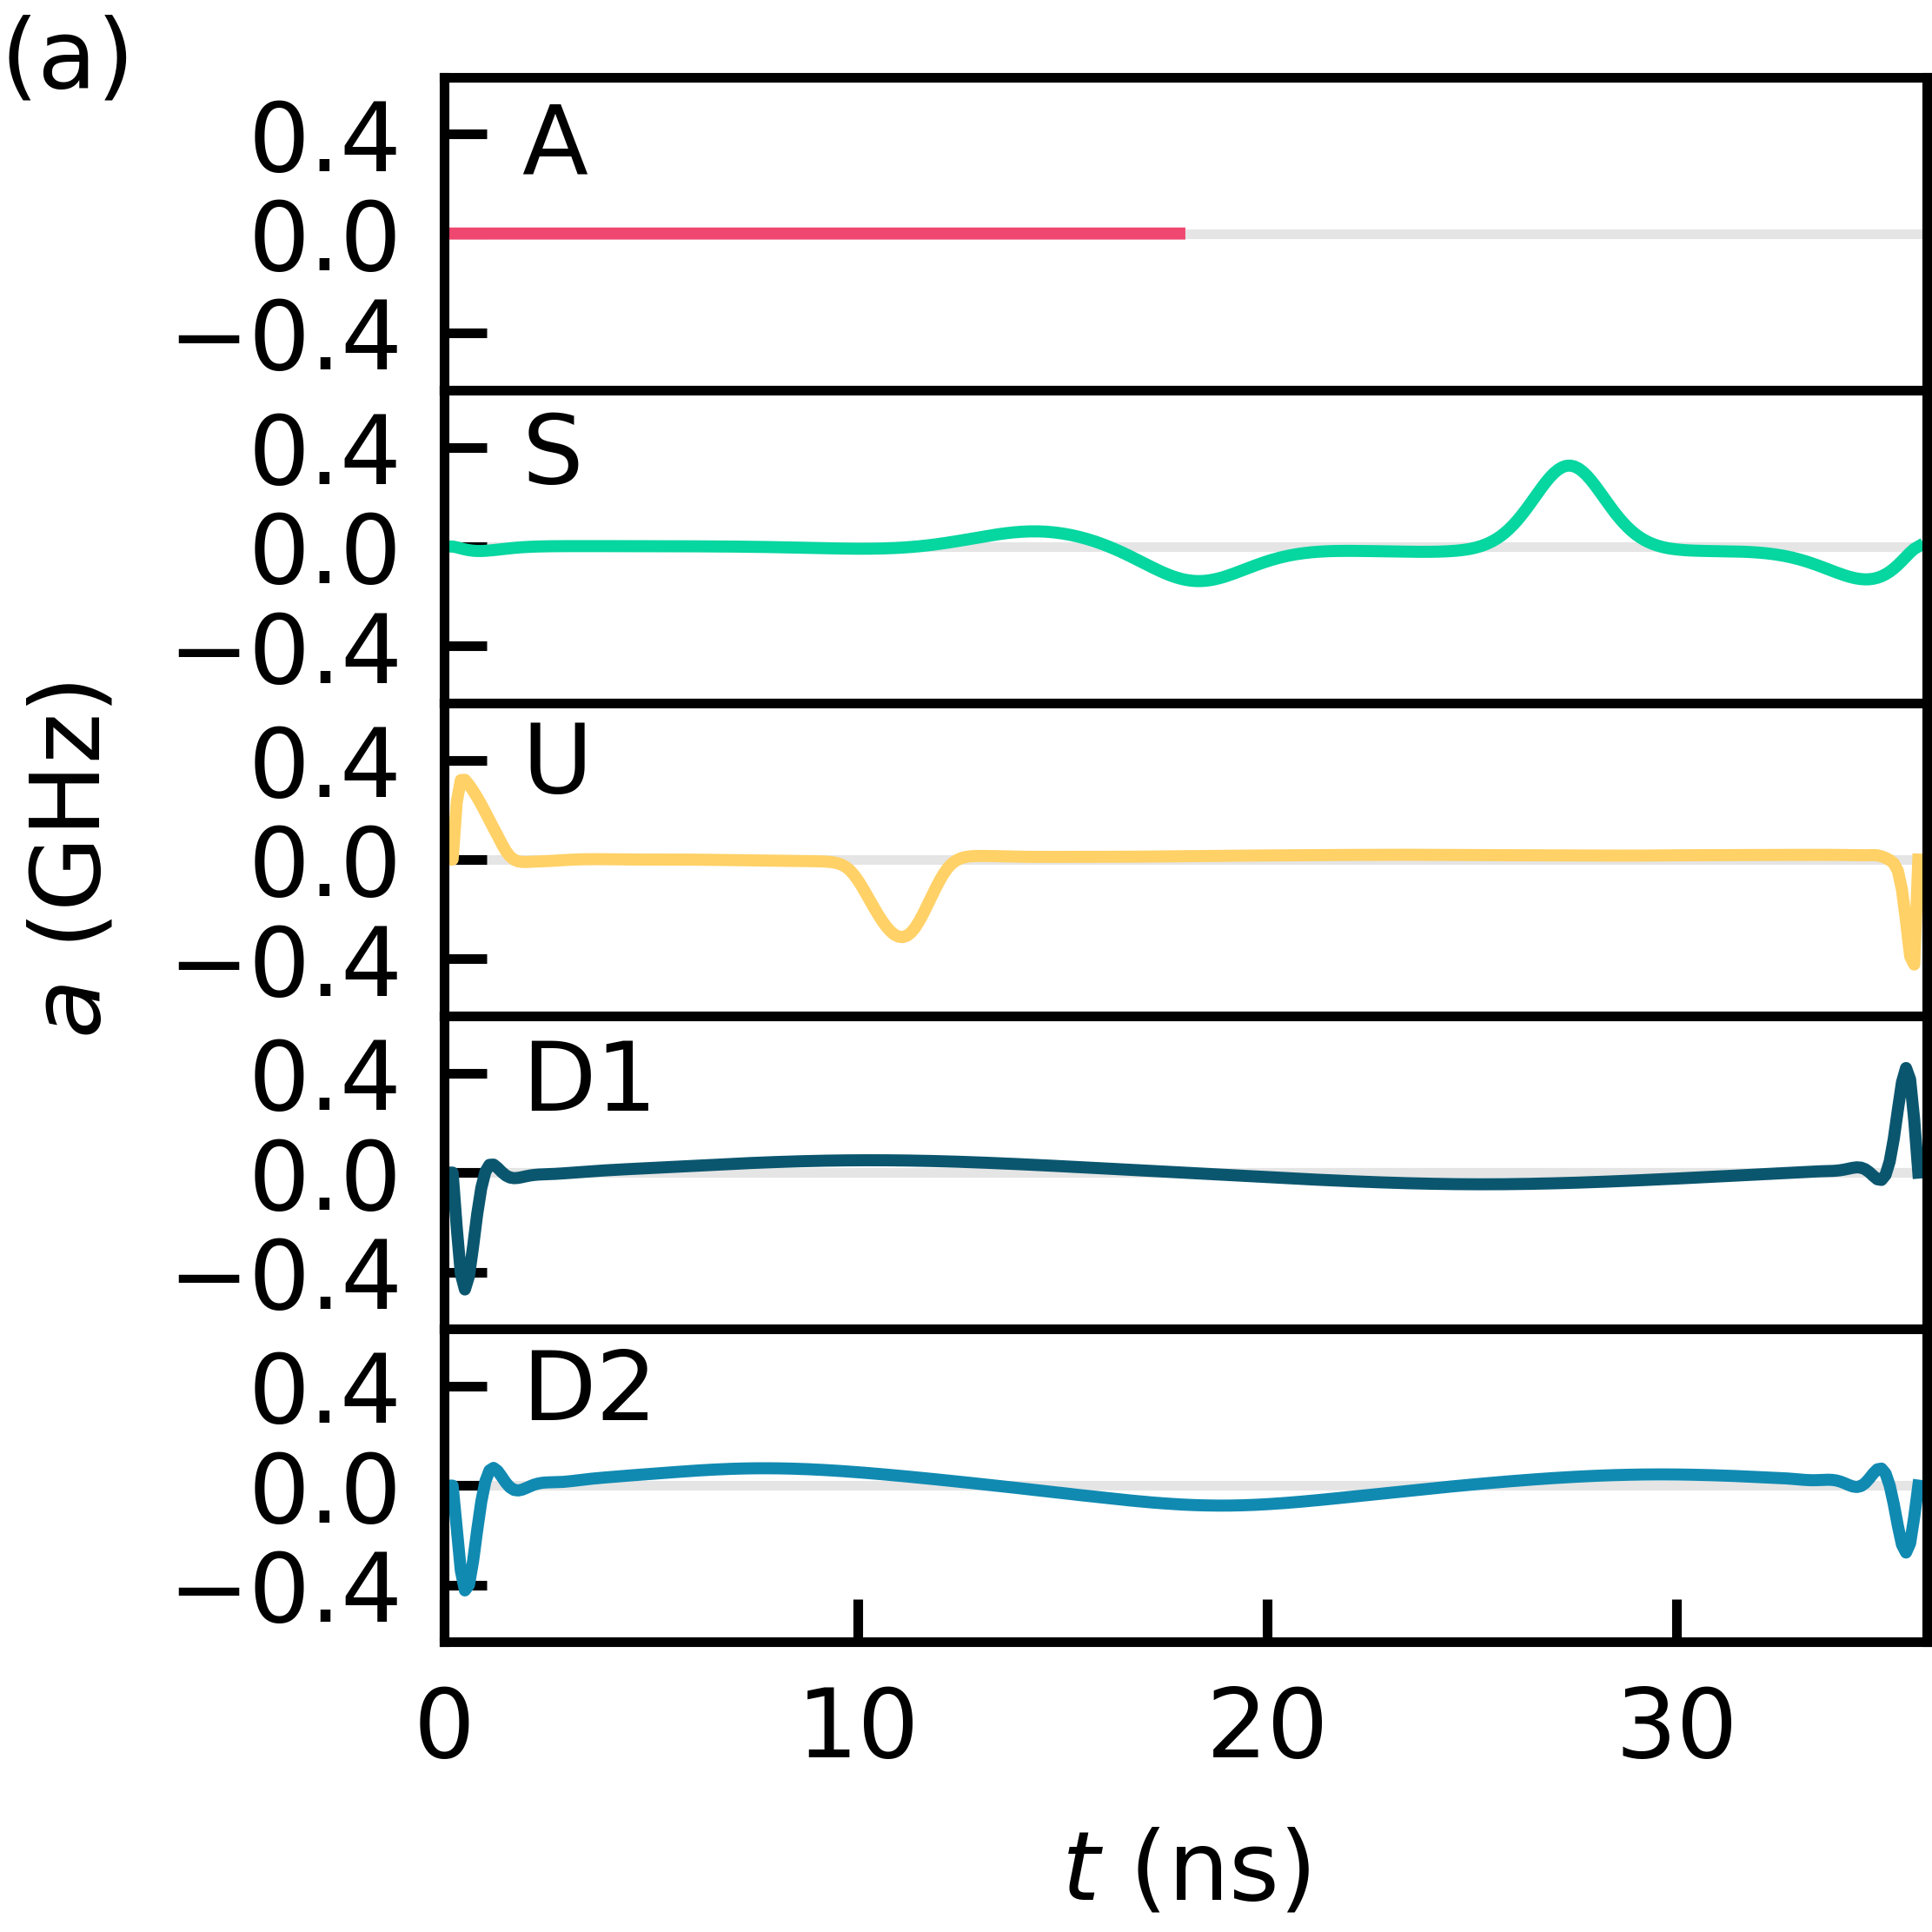
\includegraphics[width=\linewidth]{assets/f2a.png}
    \caption{\label{fig:statica}}
  \end{subfigure}\hfill
  \begin{subfigure}{.4\textwidth}
    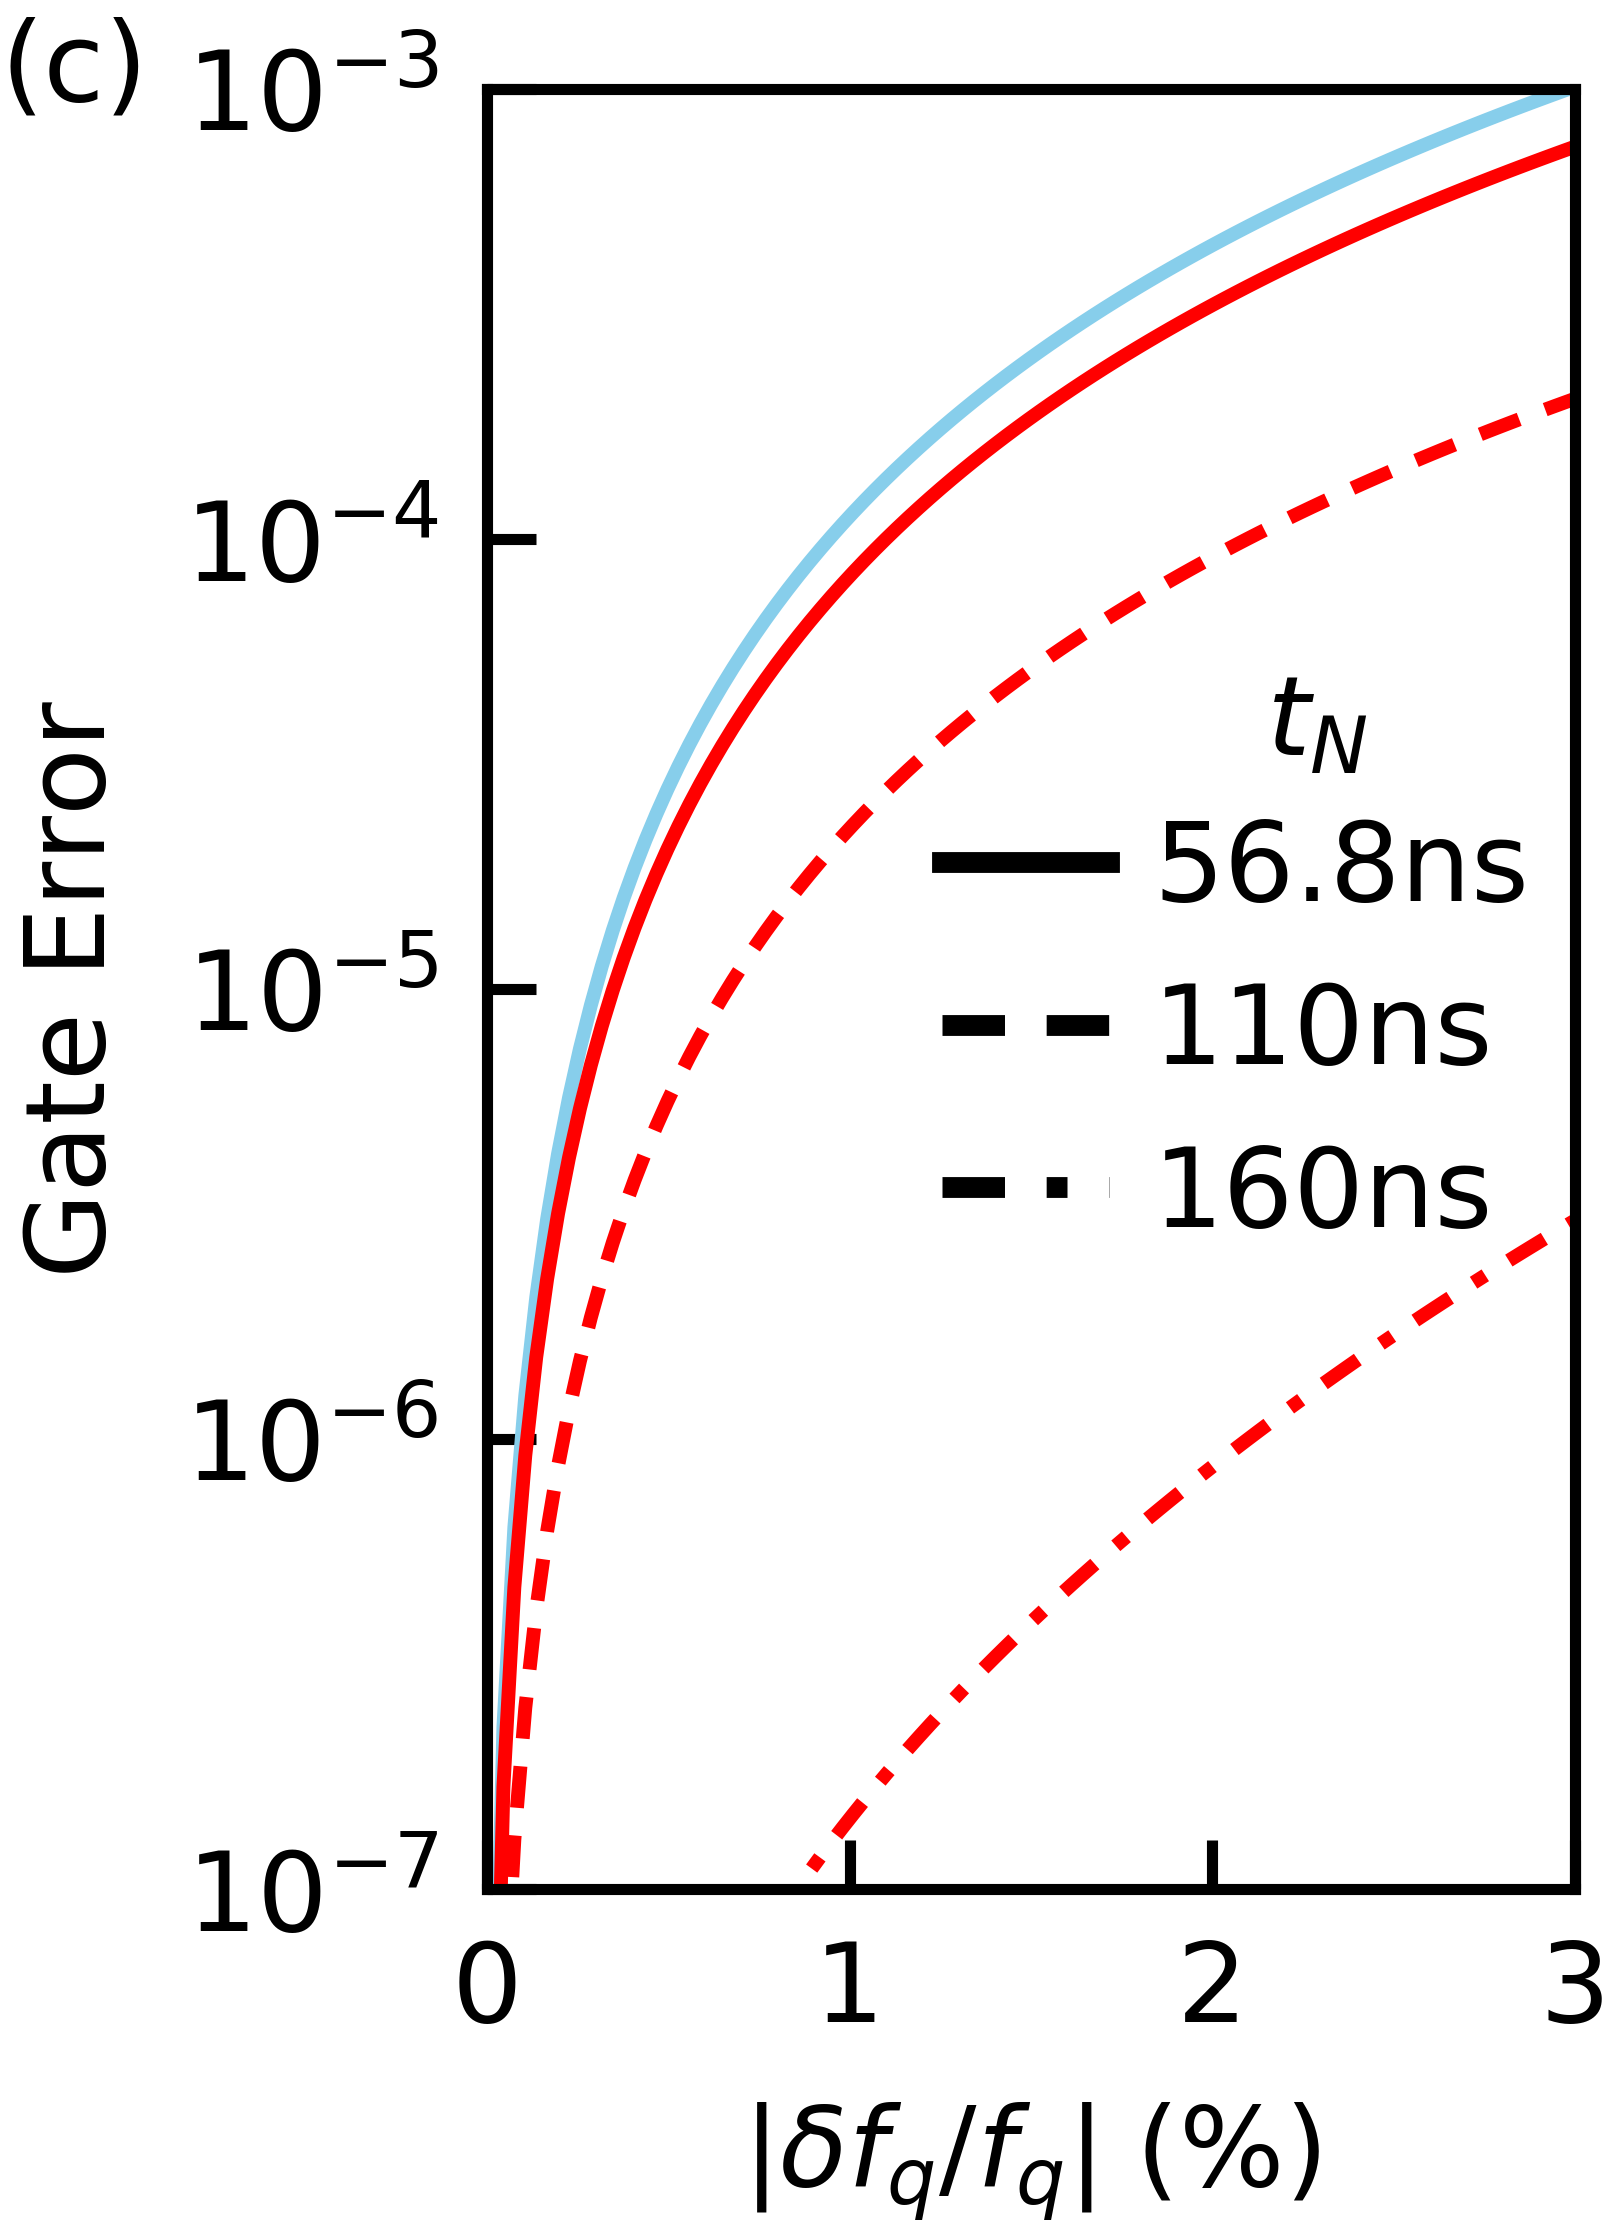
\includegraphics[width=\linewidth]{assets/f2b.png}
    \caption{\label{fig:staticb}}
  \end{subfigure}\hfill
  \begin{subfigure}{.23\textwidth}
    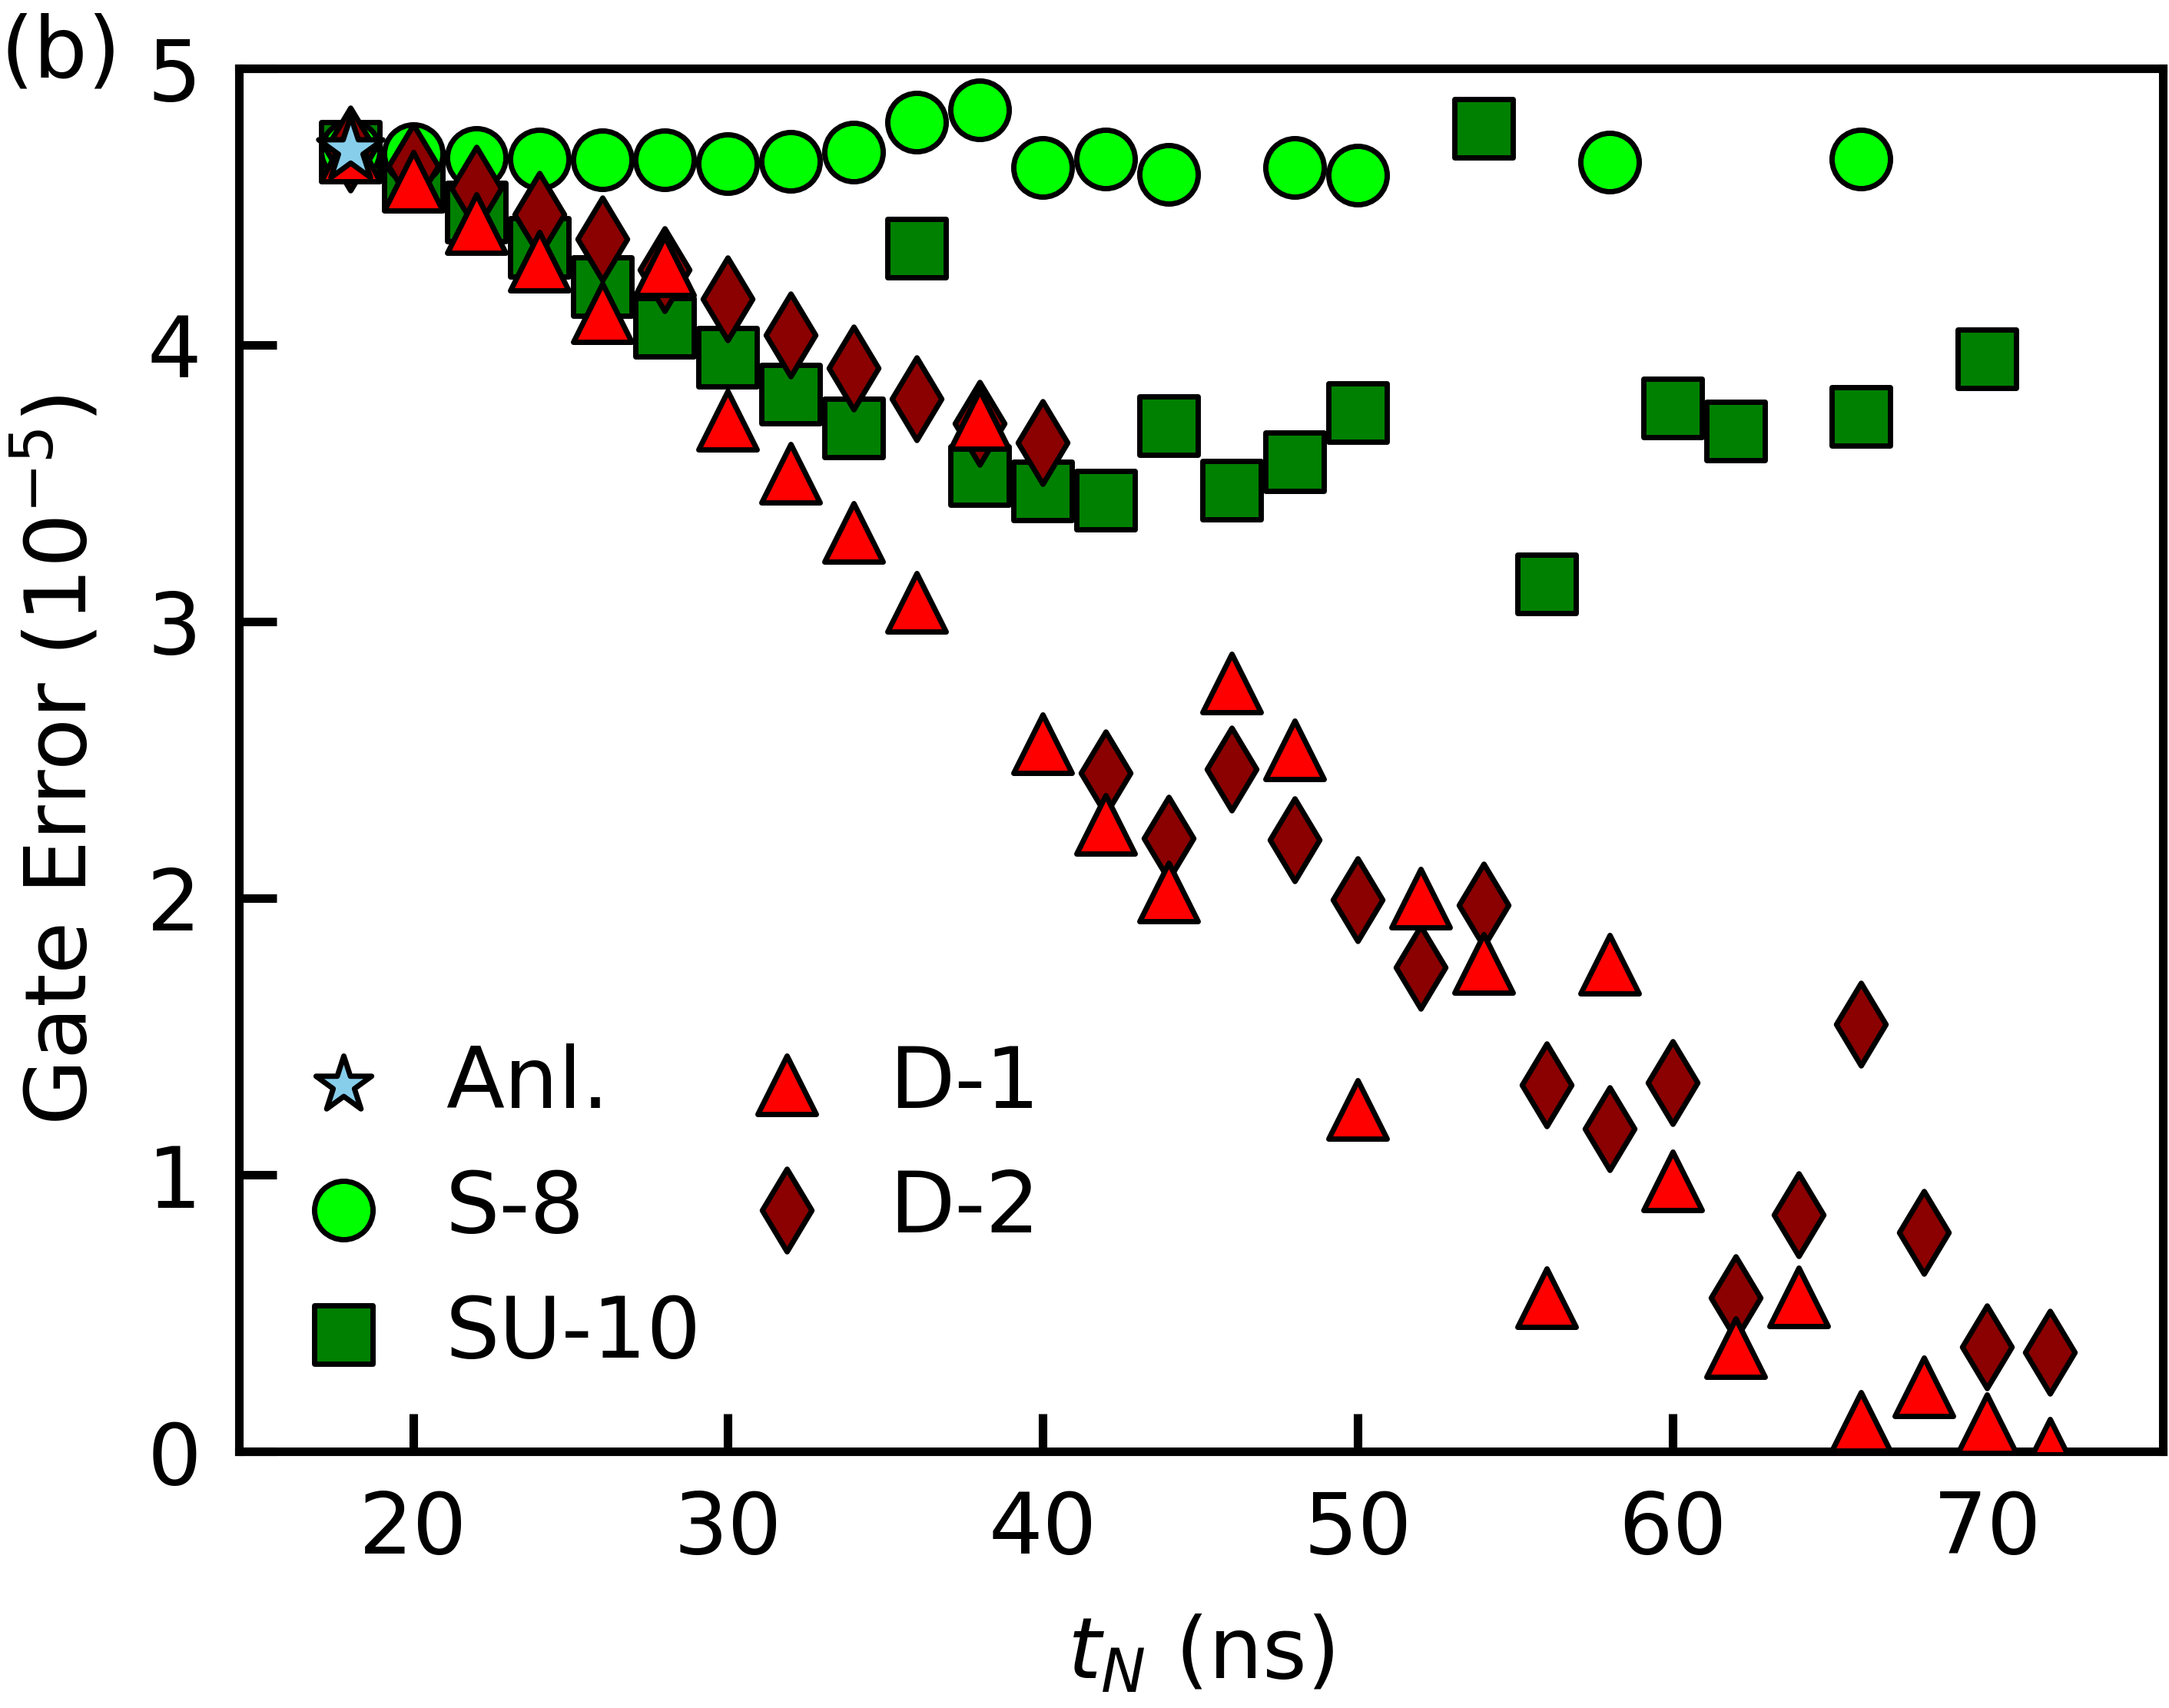
\includegraphics[width=\linewidth]{assets/f2c.png}
    \caption{\label{fig:staticc}}
  \end{subfigure}
  \caption{
    (a) Flux pulses for $Z/2$ gates robust to qubit frequency detunings constructed with the
    analytic (A), sampling (S), unscented sampling (U), and the 1\textsuperscript{st}-
    and 2\textsuperscript{nd}-order derivative methods (D1, D2). The flux pulses shown
    for the sampling, unscented sampling, and derivative methods are optimized
    for twice the gate time of the analytic gate.
    (b) Single gate error at a one-percent qubit frequency detuning as
    a function of the gate time. Missing
    data points represent gates with a gate error greater than $5 \cdot 10^{-5}$.
    (c) Single gate error as a function of the qubit frequency detuning.
    The gate errors for the analytic and 1\textsuperscript{st}-order derivative
    methods are shown for gate times which are multiples of $1 / 4 f_{q} \sim 18 \textrm{ns}$.
    The gate errors for the two methods are
    indistinguishable at the gate time $18 \textrm{ns}$.
  }
  \label{fig:static}
\end{figure*}

\section{Robustness to Static Parameter Uncertainty \label{sec:static}}
We have formulated the QOC
problem as an open-loop optimization problem; equivalently,
we do not incorporate feedback from the experiment in optimization.
However, the device's parameters deviate from the parameters we use in optimization,
leading to poor experimental performance. We combat errors
of this form using robust control techniques,
making the state evolution insensitive
to parameter uncertainty. As an example,
we mitigate errors arising from the drift and finite measurement
precision of the qubit frequency, which modifies the fluxonium Hamiltonian
\eqref{eq:hamiltonian} by $f_{q} \rightarrow f_{q} + \delta f_{q}$.
We consider three robust control techniques to accomplish this task:
a sampling method, an unscented sampling method,
and a derivative method.

The sampling method incentivizes the optimizer
to ensure multiple copies of a state, each of which evolves
with a distinct value of the uncertain parameter, achieve
the same target state. Variants of this technique have been proposed
in the context of QOC
\cite{allen2019robust, ball2020software, khaneja2005optimal,
  reinhold2019controlling, rembold2020introduction} and applied
experimentally \cite{carvalho2020error}.
For each initial state,
we add two sample states $\ket{\psi^{\pm}}$
to the augmented state \eqref{eq:astatecontrols}. The discrete dynamics
function \eqref{eq:dyn_con} is modified
so the sample states evolve under the fluxonium Hamiltonian \eqref{eq:hamiltonian}
with $f_{q} \rightarrow f_{q} \pm \sigma_{f_{q}}$ for a fixed
hyperparameter $\sigma_{f_{q}}$ which is the standard deviation of the qubit frequency.
We penalize the infidelities of the sample states and their target state
by adding a cost function to the objective \eqref{eq:costfun} of the form
$\sum_{k, \pm} b_{k} (1 - {\lvert \braket*{\psi^{\pm}_{k}}{\psi_{f}} \rvert}^{2})$
where $b_{k}$ is a constant we supply.
For this method, the standard orthonormal basis states are an insufficient choice
for the initial states. As an example, a $Z/2$ gate achieved by idling
at the flux frustration point $a_{k} = 0 \ \forall \ k$
will be robust to qubit frequency detunings for the initial states $\ket{0}$
or $\ket{1}$ because the infidelity metric is insensitive to global phases,
but this gate will not be robust for any other initial states.
Therefore, we choose four initial states
so that their outer products
span the operators on the Hilbert space
$\{\ket{0}, \ket{1}, (\ket{0} + i\ket{1}) / \sqrt{2},
(\ket{0} - \ket{1}) / \sqrt{2}\}$ \cite{chow2009randomized},
which we refer to as the operator basis.

Whereas the sampling method penalizes the deviations of the sample states
from the target state, the unscented sampling method
penalizes the deviations of the sample states from the nominal state
\cite{howell2020direct, lee2013sigma,
  thangavel2020robust}. Accordingly, the cost function we add
to the objective \eqref{eq:costfun} takes the form
$\sum_{k, j} c_{k} (\psi^{j}_{k} - \psi_{k})^{T}
(\psi^{j}_{k} - \psi_{k})$, where $c_{k}$ is a
constant we supply, $\psi_{k}$ is
the evolved initial state (nominal state), and $\psi^{j}_{k}$ is a sample state
that evolves under a modified Hamiltonian similar to that in the sampling method.
We omit bra-ket notation here to emphasize that
the states are real vectors and are given by the right-hand-side of the
complex-to-real isomorphism \eqref{eq:isomorphism}.
The sample states are chosen to encode a unimodal distribution over
the $2n$ elements of the nominal state, modeling the uncertainty in the state
as a result of the uncertainty in the parameter. We use the unscented transform
\cite{julier2004unscented, uhlmann1995dynamic}
to accurately propagate the mean and covariance of this distribution between
time steps, or equivalently, through the transformation of the TDSE \eqref{eq:tdse}.
Unlike the sampling method, the cost function for the unscented sampling method
is sensitive to global phases. Accordingly, we
do not observe a performance increase when
using more than one initial state. 
A detailed procedure for the unscented transformation is given
in Appendix \ref{appendix:unscented}.

The derivative method penalizes the sensitivity of the state
to the uncertain parameter, which is encoded in the $l$\textsuperscript{th}-order
state derivative $\ket*{\partial_{f_{q}}^{l} \psi} \equiv \partial_{f_{q}}^{l} \ket*{\psi}$.
In the $m$\textsuperscript{th}-order
derivative method, we append all state derivatives of order $1, \dots, m$
to the augmented state vector \eqref{eq:astatecontrols}
for each initial state.
We obtain the state derivatives at each time step by performing forward-mode
differentiation on the TDSE \eqref{eq:tdse}.
For example, the dynamics for the $1$\textsuperscript{st}-order derivative method are:
\begin{align}
  i \hbar \frac{d}{dt} \ket{\psi} &= H \ket{\psi},\\
  i \hbar \frac{d}{dt} \ket{\partial_{f_{q}}\psi} &=
  H \ket{\partial_{f_{q}} \psi} +
  (\partial_{f_{q}} H) \ket{\psi}.
  \label{eq:d1dyn}
\end{align}
We integrate the coupled ODEs with exponential
integrators in the discrete dynamics function \eqref{eq:dyn_con},
see Appendix \ref{appendix:derivative}.
While the state $\ket*{\psi}$ has unit norm,
the state derivatives $\ket*{\partial^{l}_{f_{q}} \psi}$ need not, as is evident
from the non-unitary dynamics \eqref{eq:d1dyn}.
We penalize the norms of the state derivatives
in the objective \eqref{eq:costfun} by setting the corresponding elements
of the target augmented state to zero. Intuitively, this corresponds to penalizing
the sensitivity of each state element to the uncertain parameter. As was the case for
the unscented sampling
method, we do not observe a performance increase when using more than one initial state
for the derivative method.
For runtimes of the three robust control techniques,
consult Appendix \ref{appendix:time}.

We examine the gate errors due to a static qubit frequency
detuning for the $Z/2$ gates obtained with the robust control techniques
and the analytic $Z/2$ gate.
To compute the gate error,
an initial state is evolved
under the fluxonium Hamiltonian \eqref{eq:hamiltonian}
two separate times with the transformations
$f_{q} \rightarrow f_{q} \pm \delta f_{q}$
at the stated qubit frequency detuning $\delta f_{q}$.
The reported gate error is the infidelity of
the evolved state and the target state averaged over
the two transformations for each of $1000$ pseudorandomly
generated initial states.
We set $\sigma_{f_{q}}/f_{q} = 1\%$
for the sampling and unscented sampling
methods.

%% F3
\begin{figure*}[ht]
  \begin{subfigure}{.4\textwidth}
    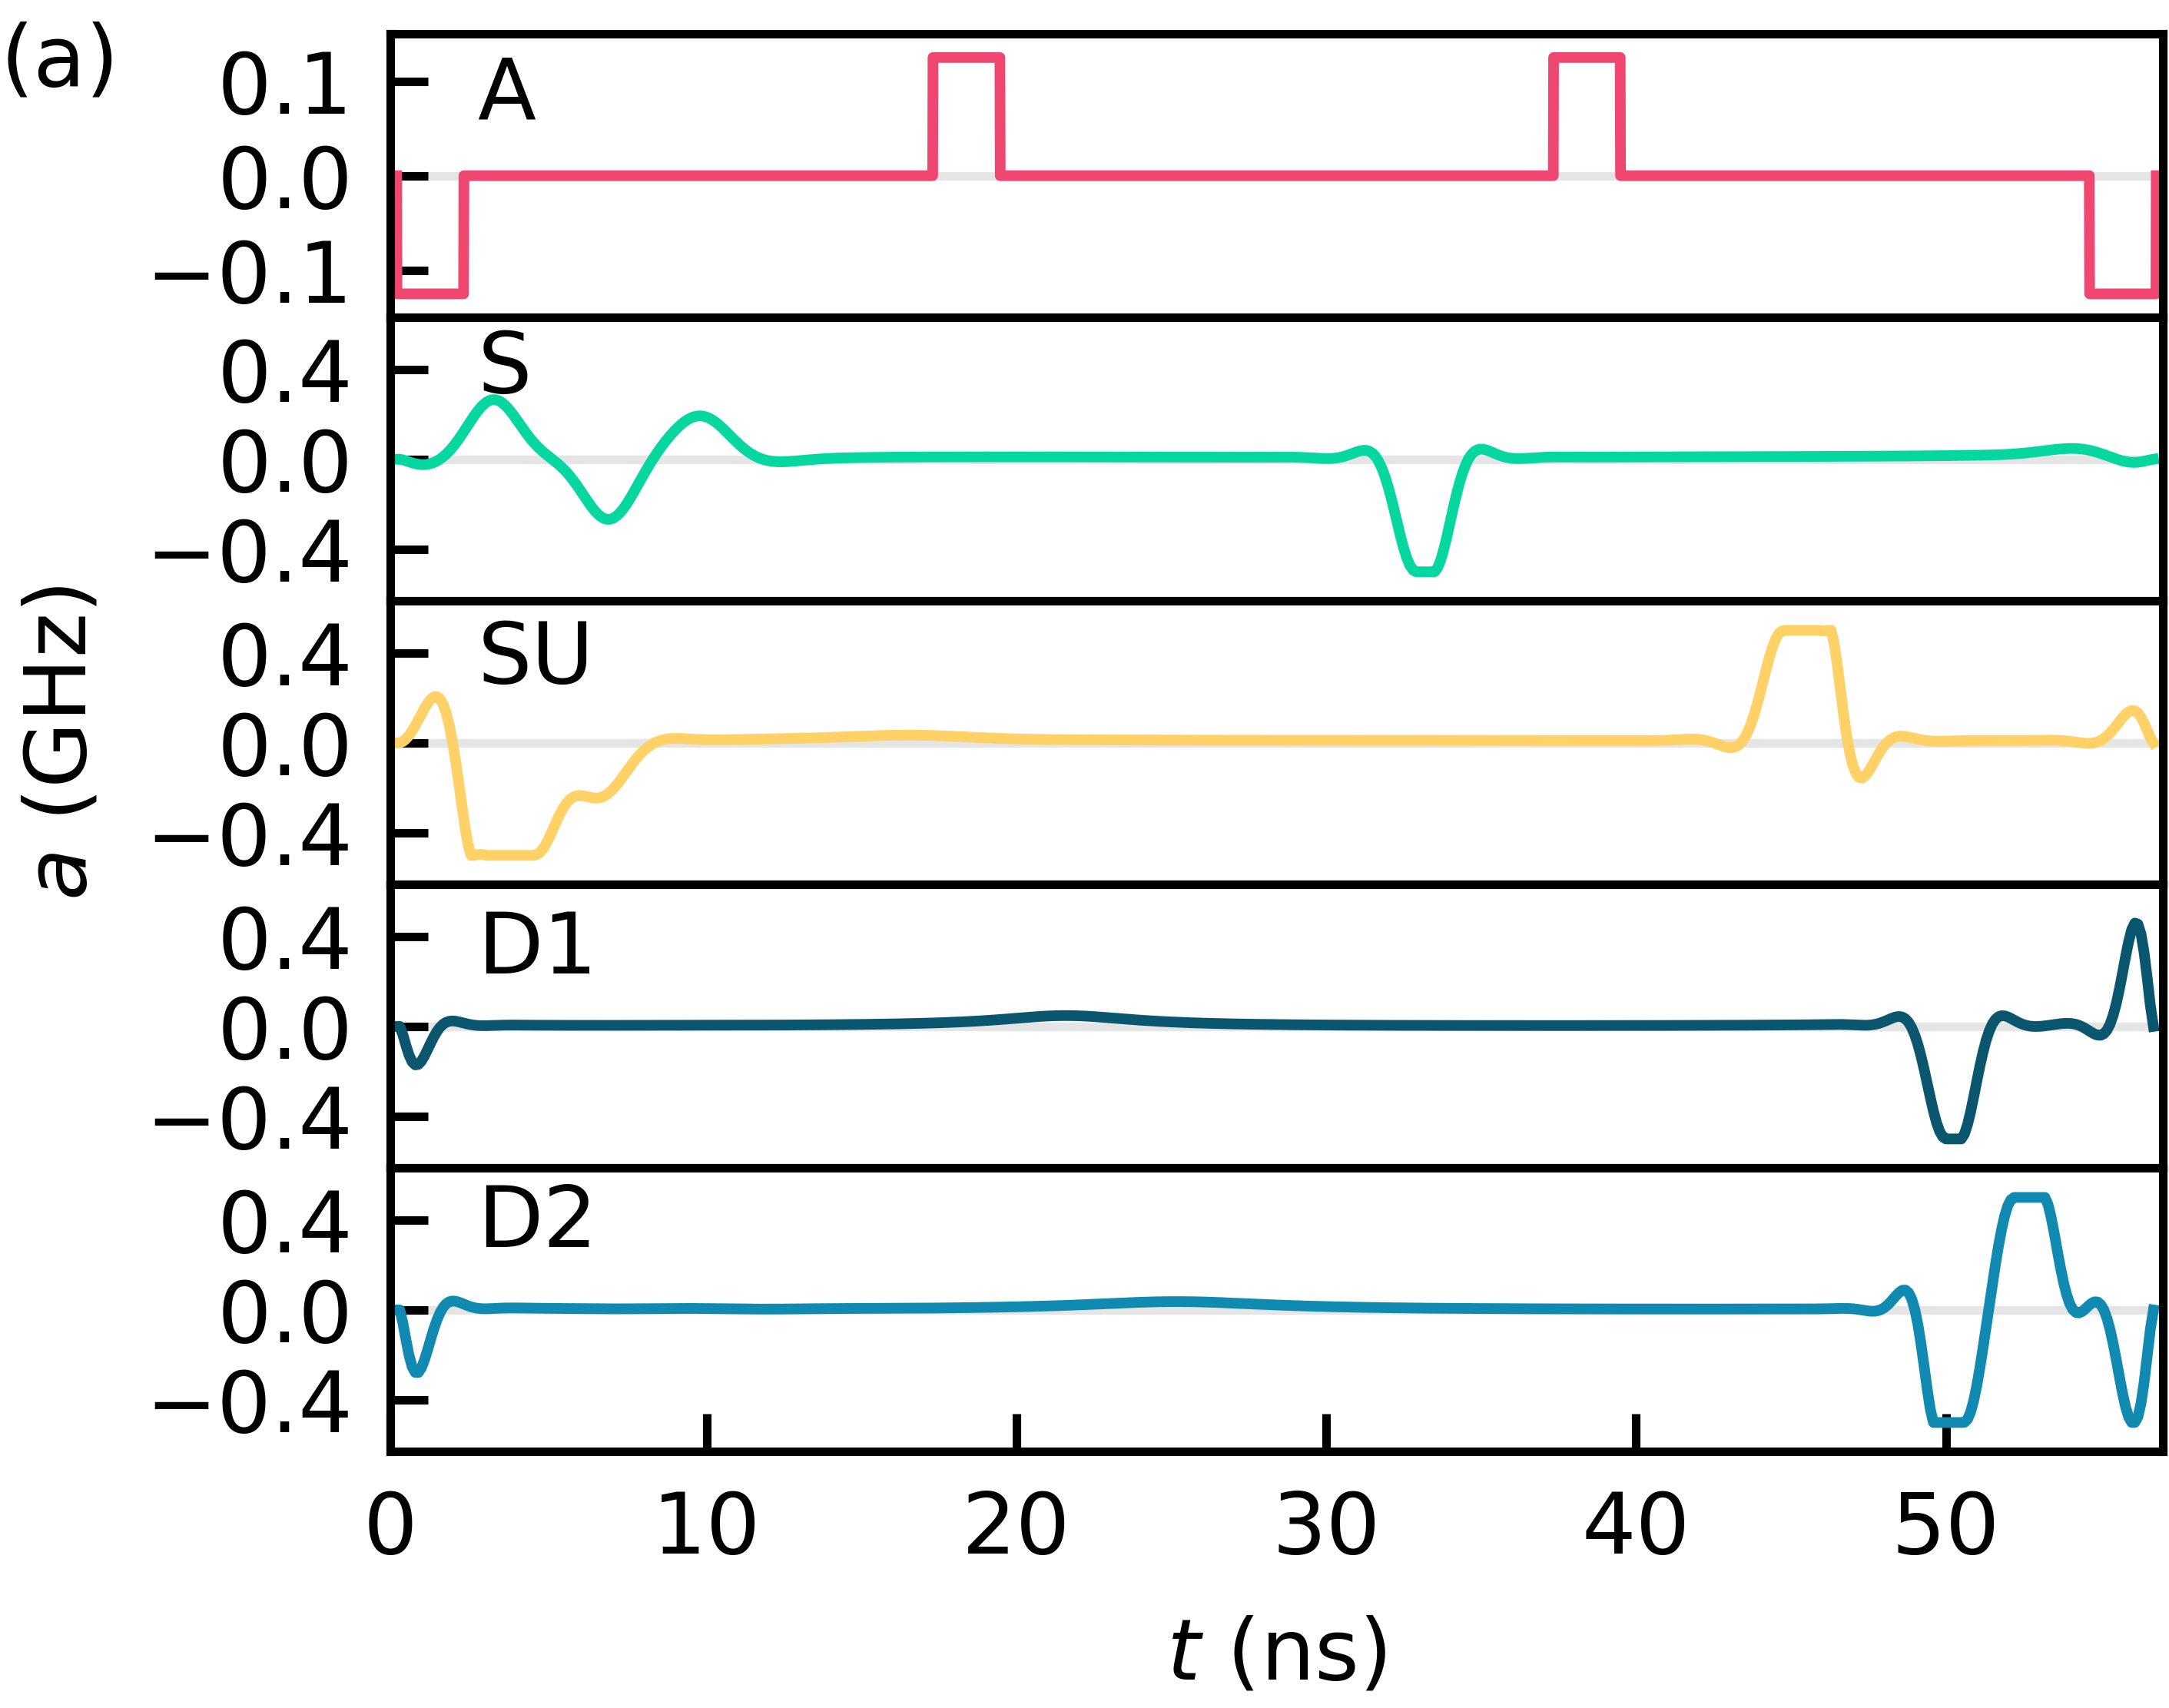
\includegraphics[width=\linewidth]{assets/f3a.png}
    \caption{}
    \label{fig:stochastica}
  \end{subfigure}\hspace{0.05\textwidth}
  \begin{subfigure}{.4\textwidth}
    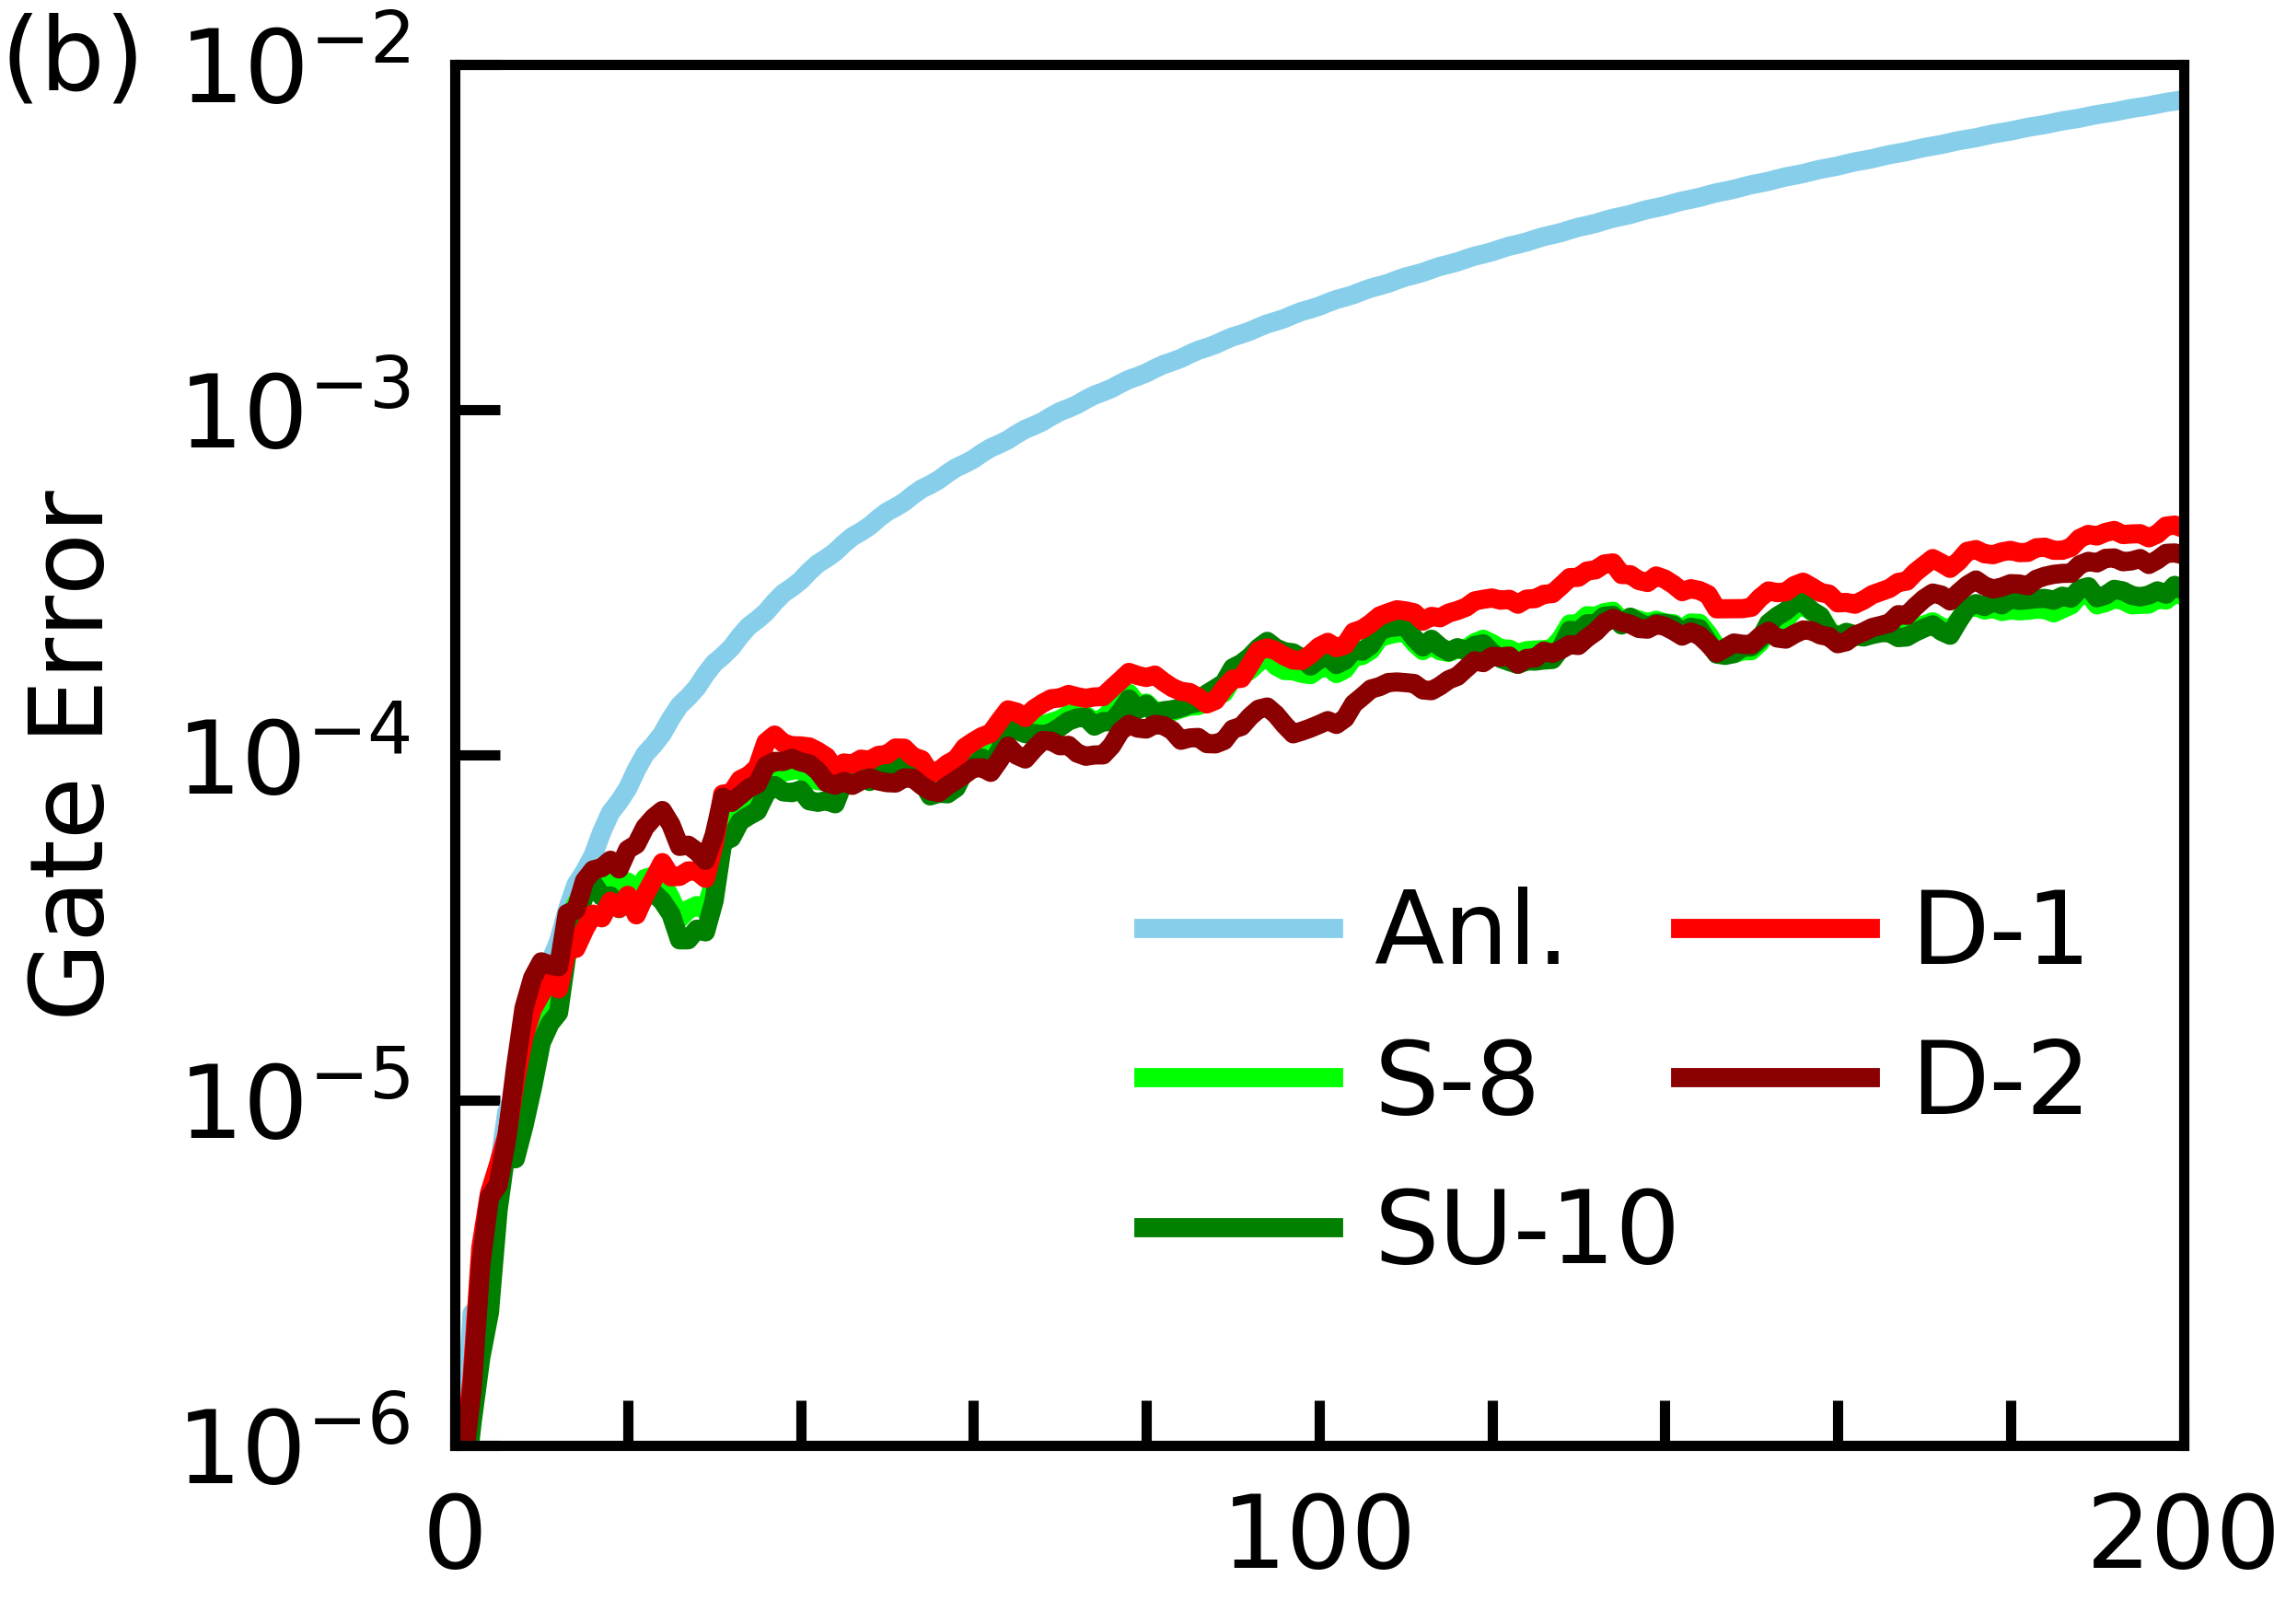
\includegraphics[width=\linewidth]{assets/f3b.png}
        \caption{}
    \label{fig:stochasticb}
  \end{subfigure}
  \caption{
    (a) Flux pulses for $X/2$ gates robust to flux noise
    constructed with the analytic (A),
    sampling (S), unscented sampling (U), and the 1\textsuperscript{st}-
    and 2\textsuperscript{nd}-order derivative methods (D1, D2).
    (b) Cumulative gate error due to 1/$f$ flux noise for
    successive gate applications. The cumulative gate errors for the
    sampling, unscented sampling, and the derivative methods are indistinguishable.
  }
  \label{fig:stochastic}
\end{figure*}

The analytic gate corresponds to
idling at the flux frustration point $a_{k} = 0 \ \forall \ k$, see Figure
\ref{fig:statica}. Its gate time $1 / 4 f_{q} \sim 18\textrm{ns}$
is the shortest possible for a $Z/2$ gate on the device.
The gate's erroneous rotation angle
$2 \pi \delta f_{q} / 4 f_{q}$ is linear in the
qubit frequency detuning, resulting in a gate error that is quadratic
in the detuning.
At a one-percent detuning $\lvert \delta f_{q} / f_{q} \rvert = 1\%$,
the gate error is $\sim 4.7 \cdot 10^{-5}$,
which is sufficient for quantum error correction.

For the sampling method, the gate error at a one-percent qubit frequency detuning
does not decrease substantially over the
range of gate times, and begins to increase above $5 \cdot 10^{-5}$ for gate times
greater than $\sim 50$ns, see Figure \ref{fig:staticb}.
Optimization results for the sampling method reveal that it is typically
able to achieve a high fidelity for
one sample $\ket{\psi^{\pm}}$,
but not the other $\ket{\psi^{\mp}}$, indicating that it is difficult for the optimizer
to make progress on both objectives.
For the unscented sampling method,
the gate error at a one-percent detuning
does not decrease substantially 
over the gate times, but it does reach
a minimum of $\sim 3.9 \cdot 10^{-5}$
near fractions of the Larmor period $2/4f_{q} \sim 36\textrm{ns}$,
$3/4f_{q} \sim 54\textrm{ns}$, $4/4f_{q} \sim 72\textrm{ns}$.

The two derivative methods converge on qualitatively similar flux pulses that
idle near the flux frustration point and use fast triangle movements at the boundaries,
similar to the flux pulse produced by the unscented sampling method.
For both derivative methods, the gate error at a one-percent qubit frequency detuning
decreases super-linearly in the gate time.
For the 1\textsuperscript{st}-order method, the gate error at a one-percent detuning 
reaches $10^{-7}$ at the Larmor period $1 / f_{q} \sim 72$ns,
see Figure \ref{fig:staticc}.
This result mimics the
ability of composite pulses to mitigate parameter uncertainty errors to arbitrary
order with sufficiently many pulses \cite{merrill2014progress}.
It is difficult to choose an appropriate composite pulse
for the problem studied here due to our Hamiltonian and experimental constraints.
We propose comparisons between composite pulses and numerical techniques
for future work.

Furthermore, the ability to perform
$Z$-type gates in any given time is critical
for synchronizing phases in multi-qubit experiments,
where the qubits have distinct
frequencies. Notably, the analytic gate studied here cannot be extended
to gate times other than $1 / 4 f_{q}$. 
We can find gates using the numerical methods at
all gate times above $18$ns, see Figure \ref{fig:staticb}.
These numerical methods offer an effective scheme for synchronizing
multi-qubit experiments.

\section{Robustness to Stochastic Parameter Deviations \label{sec:stochastic}}
An additional source of experimental error arises from stochastic, time-varying
Hamiltonian parameter deviations. For many flux-biased and inductively-coupled
superconducting circuit elements, magnetic flux noise is a significant
source of coherent errors. Magnetic flux noise
modifies the fluxonium qubit's amplitude from its nominal value by an amount $\delta a$.
It is well studied that the spectral density of $\delta a$ follows a
1/$f$ distribution for a range of devices, consisting primarily of low frequency
noise (citations needed). Analytic methods to combat flux noise
take advantage of the low frequency characteristic and
treat the noise as quasi-static, performing generalizations of the spin-echo technique
to compensate for erroneous drift. This is the strategy employed by the analytic gate
considered here.

We compare the analytic gate and those produced by
the numerical methods discussed in the previous section
on the task of realizing a $X/2$ gate subject to 1/$f$ flux noise.
The flux noise is generated by
filtering white noise sampled from a standard normal distribution with a finite
impulse response filter \cite{saspweb2011}
\footnote{\url{https://ccrma.stanford.edu/~jos/sasp/Example_Synthesis_1_F_Noise.html}}.
It is then scaled by the 
flux noise amplitude of our device $A_{\Phi} = 5.21 \mu \Phi_{0} \implies
\delta a \sim 2.5 \cdot 10^{-5} \textrm{GHz}$.
The unscented sampling method is modified so that its sampled deviations
follow a 1/$f$ distribution by carrying the state of a finite impulse response filter
in the augmented state vector. In principle the basic sampling method could be modified
similarly but we choose to sample statically at $\delta a$ for comparision. The derivative
methods require no modification from the static case. \todo{can you provide a little more 
detail on how this noise factors into the dynamics? Are you just adding some white 
noise to $a(t)$? Are you also considering uncertainty in $f_q$ at the same time?}

We simulate successive applications of the gate constructed by each method
and compute the cumulative gate error
after each application, see Figure \ref{fig:stochastic}. Both the analytic
and numerical methods achieve single gate errors
sufficient for quantum error correction. Despite converging on qualitatively different solutions, the
numerical methods perform similarly in the concatenated gate application comparision. They achieve a two
order of magnitude cumulative gate error reduction over the analytic method after $200$
gate applications $\sim 11 \mu\textrm{s}$.
1/$f$ flux noise is a signficiant source of coherent errors in NISQ applications and
these numerical techniques offer effective avenues to mitigate them.

\section{Conclusion}
In conclusion, we have applied state-of-the-art trajectory
optimization techniques to mitigate decoherence and
achieve robustness to parameter uncertainty
errors on a quantum system.
We have proposed a scheme for suppressing
depolarization with time-optimal
control and the depolarization probability model.
The computational cost of this model is
independent of the dimension of the Hilbert space, enabling
inexpensive optimization on high-dimensional quantum systems.
We have also proposed the derivative method for robust control which achieves
super-linear gate error reductions in the gate time for the static parameter
uncertainty problem we studied.
We have shown that the derivative, sampling, and unscented sampling methods
can mitigate 1/$f$ flux noise errors--which
dominate coherent errors for flux controlled qubits.
These robust control techniques can be applied
to any Hamiltonian,
allowing experimentalists in all domains to engineer robust
operations on their quantum systems.
These methods will be used to achieve the low gate errors
required for fault-tolerant quantum computing applications. Our
implementations of the techniques described in this work are available
at \url{https://github.com/SchusterLab/rbqoc}. \todo{static code?}

\begin{acknowledgments}
  We thank Helin Zhang for experimental assistance
  and Taylor Howell, Tanay Roy, Colm Ryan, and Daniel Weiss for useful discussions.
  This work is funded in part by EPiQC, an NSF Expedition in Computing, under grant CCF-1730449.
  This work was supported by the Army Research Office under Grant No. W911NF1910016.
  This work was made possible by many open source software projects,
  including but not limited to:
  Altro.jl \cite{howell2019altro},
  DifferentialEquations.jl \cite{rackauckas2017differentialequations},
  Distributions.jl \cite{besancon2019distributions},
  ForwardDiff.jl \cite{revelsLubinPapamarkou2016},
  Matplotlib \cite{hunter2007matplotlib},
  NumPy \cite{harris2020array},
  and Zygote.jl \cite{innes2018don}.
\end{acknowledgments}


\appendix
\section{Experiment}
We measure $T_{1}$ using the standard experiment
and $T_{2}$ using te Ramsey experiment. We fit with splines
and the data looks like fig. 3 in Helin's paper \cite{zhang2020universal}.
We measure $f_{q}$ and $\sigma_{f_{q}}$ using X method.

%% A1
\section{Dissipation}
To completely model the effect of longitudinal
relaxation on the quantum system we employ
the Lindblad master equation. This equation takes the form
\begin{equation}
  \frac{d}{dt} \rho = \frac{-i}{\hbar} [H, \rho] + \sum_{i = 1}^{N^{2} - 1} \gamma_{i} (L_{i} \rho L_{i}^{\dagger} - \frac{1}{2} \{L_{i}^{\dagger} L_{i}, \rho\})
\end{equation}
where $\rho = \ket{\psi}\bra{\psi}$ is the density matrix, $N = \textrm{dim}(\mathcal{H})$,
and $[\cdot, \cdot], \{\cdot, \cdot \}$ are the algebraic commutator and anti-commutator.
For longitudinal relaxation $\gamma_{1} = T_{1}^{-1} = T_{1, \uparrow}^{-1} + T_{1, \downarrow}^{-1}$
and $L_{\uparrow} = \sigma^{+}/2$,
$L_{\downarrow} = \sigma^{-}/2$
are the ladder operators $\sigma^{\pm} = \sigma_{x} \pm i \sigma_{y}$. For pure dephasing
$\gamma_{2} = T_{2}^{-1} = (2 T_{1})^{-1} + T_{\phi}^{-1}$ and
$L_{2} = (I - \sigma_{z})/2$.

%% T1
\begin{table}[ht]
  \begin{tabular}{c | c | c | c | c | c | c}
         & Analytic & QOC & & Analytic & QOC & \\
    Gate & $P_{1}\ (10^{-5})$ & $P_{1}\ (10^{-5})$ & $P_{1\textrm{A}} / P_{1\textrm{Q}}$
    & GE $(10^{-5})$ & GE $(10^{-5})$ & GE$_{\textrm{A}}$ / GE$_{\textrm{Q}}$\\
    \hline
    Z/2 & 5.745  & 1.149 & 5.000 & 1.776 & 0.371 & 4.787\\
    Y/2 & 5.253  & 1.157 & 4.540 & 1.539 & 0.370 & 4.159\\
    X/2 & 16.251 & 2.660 & 6.109 & 5.347 & 0.863 & 6.196\\
  \end{tabular}
  \caption{Probability of longitudinal relaxation for each gate
    evaluated at the gate's duration.}
\end{table}

\section{Derivative Method}
\label{appendix:derivative}
We comment on the optimization metrics of the derivative methods and then
outline how to efficiently integrate their dynamics.
The 1\textsuperscript{st}-order derivative method tends
to outperform the 2\textsuperscript{nd}-order
derivative method in the small, static detuning regime, see Figure \ref{fig:static}b.
The norms of the state derivatives for the 1\textsuperscript{st}- and 2\textsuperscript{nd}-order
methods are provided in Table \ref{tab:dnorm} for the solutions at $t_{N} = 60$ns.
The 2\textsuperscript{nd}-order method is able to decrease the 2\textsuperscript{nd}-order
state derivate norm relative to the 1\textsuperscript{st}-order method at the expense of increasing
its 1\textsuperscript{st}-order derivative norm. In the problem
we have studied it is likely the 2\textsuperscript{nd}-order derivative norm has a smaller
contribution to the gate error than the 1\textsuperscript{st}-order derivative norm. A
careful analysis could be completed for future problems to predict the efficacy of the
derivative method at each order.

\begin{table}[h]
  \begin{tabular}{c | c | c}
    Method & ${\lvert \braket{\partial_{f_{q}} \psi_{N} | \partial_{f_{q}} \psi_{N}} \rvert}^{2}$ ($10^{3}$)
    & ${\lvert \braket{\partial^{2}_{f_{q}} \psi_{N} | \partial^{2}_{f_{q}} \psi_{N}} \rvert}^{2}$ ($10^{6}$)\\
    \hline
    D-1 & 0.436 & 57.817\\
    D-2 & 1.702 & 9.030\\
  \end{tabular}
  \caption{Norm of state derivates with respect to the qubit frequency
    for $Z/2$ gates optimized using the derivative methods. The norms are computed
    at the end of the gate's duration $t_{N} = 60$ns and are averaged over the four state derivatives.}
  \label{tab:dnorm}
\end{table}

The dynamics for the derivative methods can be integrated efficiently using exponential integrators
\cite{berland2005solving, einkemmer2017performance}.
General exponential integrators break the dynamics into a linear term and a non-linear term. For example, consider
integrating the dynamics of the first state derivative $\frac{d}{dt} \ket{\partial_{\lambda} \psi} =
H \ket{\partial_{\lambda} \psi} + (\partial_{\lambda} H) \ket{\psi}$ in units of $i\hbar = 1$.
The linear term is $L = H$ and the non-linear term is $N = (\partial_{\lambda} H) \ket{\psi}$.
With zero-order hold on the controls the exact propagation is
\begin{equation}
  \label{eq:dgeneralexp}
  \begin{aligned}
    \ket{\partial_{\lambda} \psi_{k + 1}} &= \exp(\Delta t_{k} L_{k}) \ket{\partial_{\lambda} \psi_{k}}\\
    &+ \int_{0}^{\Delta t_{k}} \exp((\Delta t_{k} - t^{'})L_{k}) N(t_{k} + t^{'}) dt^{'}\\
  \end{aligned}
\end{equation}
General exponential integrators proceed by breaking the integral in \eqref{eq:dgeneralexp}
into a discrete sum, similar to the procedure
for Runge-Kutta schemes. We use a simple approximation known as the Lawson-Euler
method \cite{berland2005solving}
\begin{equation}
  \begin{aligned}
    \ket{\partial_{\lambda} \psi_{k + 1}} &\approx \exp(\Delta t_{k}L_{k}) \ket{\partial_{\lambda} \psi_{k}}\\
    &+ \exp(\Delta t_{k}L_{k}) N_{k}\\
  \end{aligned}
\end{equation}
This method provides a good tradeoff between accuracy and efficiency, requiring one unique matrix
exponential computation per stage. Integration accuracy is not of the utmost importance because the
state derivatives guide the optimization, and do not correspond to experimental parameters
which must be realized with high accuracy.





%% AE
\section{Complex Tensor Handling}
We use an isomorphism $\mathcal{H}(\mathbb{C}^{n}) \cong \mathcal{H}(\mathbb{R}^{2n})$
because the software we use does not support complex numbers yet.



\bibliography{refs}

\end{document}
